\documentclass[a4paper, 12pt]{book}
\includeonly{introduction, chapter01, chapter02, chapter03}
\usepackage[a4paper, BCOR1cm]{typearea}
\usepackage[spanish, es-ucroman]{babel}
\usepackage[format=hang, font=small, labelfont=bf, labelsep=endash, width=.9\textwidth]{caption}
\usepackage[listofformat=subsimple, format=hang, labelfont=footnotesize, textfont={it, footnotesize}]{subfig}
\usepackage[color]{changebar}
\usepackage[latin1]{inputenc}
\usepackage[OT1]{fontenc}
\usepackage[bf, sf]{titlesec}
\usepackage[nottoc]{tocbibind}
\usepackage[spanish]{varioref}
\usepackage{graphicx}
\usepackage{amsfonts, amsmath, amssymb, calc, color, fancyhdr, hyperref, ifthen, listings, nextpage, textcase}
\usepackage{array, booktabs, tabularx, tabulary, dcolumn, multirow, threeparttable}
\titleformat{\part}[display]{\centering\huge\sffamily\bfseries}{\partname\ \thepart}{.5\baselineskip}{}
\hypersetup{%
	pdftitle=Proceso de adquisici�n y tratamiento de se�ales de %
	ultrasonidos, pdfauthor=Jos� Ram�n Gisbert Valls, pdfcreator=Vim 7.2,%
	pdfstartview=FitH, colorlinks=true, pdfdisplaydoctitle=true,%
	naturalnames=true, breaklinks=true, linkcolor=black,%
	bookmarksopen=true, bookmarksopenlevel=1
}
\fancyhf{}
\fancyhead[RO, LE]{\sffamily\bfseries\thepage}
\fancyhead[LO]{\sffamily\nouppercase{\rightmark}}
\fancyhead[RE]{\sffamily\nouppercase{\leftmark}}
\pagestyle{fancy}
\fancypagestyle{plain}{%
	\fancyhf{}
	\renewcommand\headrulewidth{0pt}
}
\lstloadlanguages{Matlab}
\lstset{language=Matlab, extendedchars=true, breaklines}
\cbcolor{red}
\labelformat{equation}{ecuaci�n~#1}
\labelformat{figure}{figura~#1}
\labelformat{section}{secci�n~#1}
\labelformat{subsection}{secci�n~#1}
\labelformat{subsubsection}{secci�n~#1}
\labelformat{table}{cuadro~#1}
\labelformat{footnote}{#1\protect\iscurrentchapter{\thechapter}}
\setkeys{Gin}{width=.8\textwidth}
\graphicspath{{./pictures/}{../pictures/}}
\DeclareCaptionLabelFormat{cont}{#1~#2\alph{ContinuedFloat}}
\captionsetup[ContinuedFloat]{labelformat=cont}
\newcommand\matlab{\textsc{matlab}}
\newcommand\kpci{\textsc{kpci}-3108}
\newcommand\datx{\emph{Data Acquisition Toolbox}}
\newcommand\iscurrentchapter[1]{\ifthenelse{\equal{#1}{\thechapter}}{  en el Cap�tulo~#1}}
\newcommand\miniit[1]{\begin{itemize} #1 \end{itemize}}
\newcommand\tnotetext[2]{\item\hspace*{-5pt}\raisebox{.7ex}{\fontsize{7pt}{8.4pt}\selectfont\normalfont #1}{\footnotesize #2}}
\newenvironment{TableNotes}{\begin{tablenotes}\vspace{\footnotesep}\footnoterule\vspace{.2ex}}{\end{tablenotes}}
\renewcommand\chaptermark[1]{\markboth{#1}{}}
\renewcommand\cleardoublepage{\cleartooddpage[\thispagestyle{empty}]}
\newcolumntype{d}[1]{D{,}{,}{#1}}
\newcolumntype{+}{D{/}{\mbox{\ --\ }}{5}}
\begin{document}

\frontmatter

\tableofcontents

\listoftables

\listoffigures

\chapter{Introducci�n}

Una de las aplicaciones industriales de los ultrasonidos es la caracterizaci�n interna de materiales. De entre las distintas t�cnicas empleadas con dicha finalidad, la inspecci�n mediante ultrasonidos ha demostrado encontrarse entre las m�s fiables. Adem�s, debido a su naturaleza esta t�cnica es, obviamente, no destructiva. El procedimiento de medida habitual consiste en hacer incidir un haz de ondas de alta frecuencia ---generalmente entre los 40 KHz y 25 MHz--- sobre la superficie de la muestra, posteriormente se registra la onda que atraviesa el material y se miden uno o varios de sus par�metros. De este modo es posible determinar la presencia de defectos tales como grietas, o la inclusi�n de materiales extra�os, en el interior de la muestra.


\section*{Objetivos del proyecto fin de carrera}\label{sec:goals}

Con objeto de explotar esta tecnolog�a, principalmente en la caracterizaci�n de bloques de madera de palmera, este proyecto pretende inicialmente la creaci�n de un sistema electr�nico de medida. Este sistema constar� de dos partes diferenciadas: 
\begin{itemize}
	\item Un sistema de adquisici�n y procesado de se�ales.
	\item Y el conjunto formado por un transmisor y un sensor de ultrasonidos junto con sus respectivos circuitos acondicionadores.
\end{itemize}


\section*{Estructura de este documento}

Debido a la independencia entre los dos bloques de que se compone el sistema de medida, se ha cre�do conveniente dividir este documento en dos partes distintas. En la primera parte se expone el procedimiento seguido durante el acondicionamiento del sistema de adquisici�n y procesado. La segunda se ocupa de dar unas breves nociones de teor�a general de ultrasonidos, justificar cual debiera ser el equipo �ptimo para realizar los experimentos, y discutir los resultados obtenidos.



\mainmatter

\part{Sistema de adquisici�n y procesado de se�ales}

\chapter{Tarjeta de adquisici�n de se�ales}

Para preparar el sistema de adquisici�n y procesado de se�ales se dispuso en origen de una tarjeta de adquisici�n con interfaz \textsc{pci}. En concreto se ha empleado el modelo \kpci{} de la casa \emph{Keithley}. A continuaci�n se exponen las caracter�sticas t�cnicas que ofrece este dispositivo, en apartados siguientes una breve descripci�n funcional y la disposici�n y uso de los puertos presentes en el mencionado dispositivo.


\section{Caracter�sticas t�cnicas del hardware}\label{sec:technical-features}

La tarjeta \kpci{} puede emplearse para la adquisici�n y conversi�n de se�ales anal�gicas en se�ales digitales, para sintetizar se�ales anal�gicas a partir de se�ales digitales previamente generadas o almacenadas, o ---gracias a sus 32 puertos digitales de prop�sito general--- trabajar con se�ales digitales.\par
El primer bloque del sistema electr�nico de medida propuesto, es decir el sistema de adquisici�n y procesado de se�ales, tan s�lo requiere de la funci�n de adquisici�n anal�gica de la tarjeta. Por ello, de entre todas las caracter�sticas del dispositivo, se ha cre�do conveniente resumir a continuaci�n aquellas que tienen relaci�n directa con dicha funci�n. Para obtener informaci�n detallada sobre la relaci�n que estos atributos guardan con el proceso de adquisici�n de se�ales anal�gicas en la tarjeta \kpci{}, rec�rrase a la \vref{sec:functional-description}.

\begin{itemize}
	\item El m�dulo de adquisici�n anal�gica dispone de 16 puertos f�sicos.
	\item La impedancia de entrada equivalente de cada puerto es aproximadamente igual a una capacidad de 200 pF en serie con una resistencia de valor inferior, pero aproximadamente igual, a 1 K$\Omega$.
	\item En condiciones �ptimas, es posible conseguir un rendimiento m�ximo de 100 KS/s (cien mil operaciones de conversi�n por segundo). Este valor est� sujeto a un error relativo del $0.02 \%$.
	\item La resoluci�n del conversor anal�gico digital es de 16 bits por muestra. El rango de amplitudes en el que opera depende de como est� configurado el modo de adquisici�n.% Este puede ser de 0 a 10 si el modo de adquisici�n es unipolar, o de -10 a 10 si es bipolar.
	\item La cola de muestreo tiene capacidad para hasta 256 canales distintos. Cada uno de los cuales puede configurarse independientemente en t�rminos de ganancia, frecuencia de muestreo, modo de adquisici�n o modo de terminaci�n.
	\item La ganancia, responsable en parte de la resoluci�n con la que se cuantifica las muestras, puede tomar cada ciclo de reloj uno de entre 16 valores posibles. V�ase el \vref{tab:acquisition-modes}.
	% \item Soporte, tanto en el modo de adquisici�n y conversi�n como en el modo de s�ntesis, para disparo digital externo o controlado por software.
	% \item Selecci�n por software del flanco activo de disparo.
	% \item Capacidad de interrumpir el muestreo tras un determinado n�mero de ciclos despu�s del disparo. La cantidad de ciclos puede controlarse por software.
\end{itemize}


\section{Descripci�n funcional}\label{sec:functional-description}

Es necesario programar el comportamiento de la tarjeta de adquisici�n antes de ponerla en funcionamiento. Desde la cola de muestreo se controlan los principales aspectos del proceso de adquisici�n, como por ejemplo, en que instantes se encuentra activo.\par% La configuraci�n correspondiente al proceso de adquisici�n anal�gica reside en su pr�ctica totalidad en la cola de muestreo. Desde la cola se controlan los principales aspectos de este proceso, como por ejemplo, en que instantes se encuentra activo.\par
La cola de muestreo, como su propio nombre indica, es una estructura de datos ordenada. Se encuentra almacenada en una memoria \textsc{ram} de 256 entradas que forma parte del hardware de la tarjeta. En el \vref{tab:sample-queue} puede verse una representaci�n de un ejemplo de la cola de muestreo.\par

\begin{table}[h]
	\centering
	\begin{threeparttable}
	\begin{tabular}{lccccccccc}
		\toprule
		Posici�n en la cola & 1 & 2 & 3 & 4 %
		& \multicolumn{2}{c}{$\cdots$} & 254 & 255 & 256 \\
		\midrule
		N�mero de canal & 15 & 15 & 02 & 02 %
		& \multicolumn{2}{c}{$\cdots$} & 17 & 13 & 01 \\
		N�mero de puerto\tnote{a, b} & 07 & 07 & 11 & 11 %
		& \multicolumn{2}{c}{$\cdots$} & 07 & 09 & 01 \\
		Ganancia & 1 & 1 & 40 & 40 %
		& \multicolumn{2}{c}{$\cdots$} & 200 & 8 & 80 \\
		Modo de adquisici�n\tnote{c} & $\pm$ & $\pm$ & $+$ & $+$ %
		& \multicolumn{2}{c}{$\cdots$} & $\pm$ & $+$ & $\pm$ \\
		Modo de terminaci�n\tnote{d} & \textsc{d} & \textsc{d} & \textsc{ts} %
		& \textsc{ts} & \multicolumn{2}{c}{$\cdots$} & \textsc{d} & \textsc{ts} %
		& \textsc{ts} \\
		\bottomrule
	\end{tabular}
	\begin{TableNotes}
		\tnotetext{a}{Si el canal es diferencial el n�mero de puerto identifica un par de puertos. Un canal diferencial no puede estar asociado a un n�mero de puerto superior a 07.}
		\tnotetext{b}{Dos canales pueden estar relacionados con los mismos puertos f�sicos.}
		\tnotetext{c}{$\pm$ configuraci�n bipolar; $+$ configuraci�n unipolar}
		\tnotetext{d}{\textsc{d} canal diferencial; \textsc{ts} canal monoterminal}
	\end{TableNotes}
	\end{threeparttable}
	\caption{Ejemplo de cola de muestreo}
	\label{tab:sample-queue}
\end{table}

Cada entrada en la memoria \textsc{ram} se identifica con una posici�n en la cola. Las posiciones en la cola pueden encontrarse vac�as o estar ocupadas por un canal. Varias posiciones en la cola, consecutivas o no, pueden estar ocupadas por un mismo canal. Por tanto, la cola puede estar ocupada, como m�ximo, por 256 canales independientes.\par
Las posiciones ocupadas contienen informaci�n correspondiente al canal y a los atributos asociados a este. Un canal es una entidad l�gica que relaciona un puerto f�sico con un b�ffer de informaci�n y una serie de atributos. Durante el proceso de adquisici�n un puntero recorre las distintas posiciones de la cola, una a una y en orden. El canal activo, aquel que ocupa la posici�n a la que apunta el puntero en cada ciclo de reloj, determina tres cosas:

\begin{itemize}
	% \footnote{Por convenio se ha elegido hablar de una sola se�al que entra al amplificador. Si se ha hecho esta elecci�n, es porque si bien al amplificador pueden entrar una o dos se�ales simult�neamente desde sendos puertos, tal y como se ver� m�s adelante, esto no supone otra diferencia para el proceso que la expuesta en la secci�n \vref{sec:termination-modes}
	\item De qu� puerto debe proceder la se�al anal�gica\footnote{Por convenio se ha elegido hablar de una sola se�al que entra al amplificador. Si se ha hecho esta elecci�n, es porque si bien al amplificador pueden entrar una o dos se�ales simult�neamente, esto no supone otra diferencia para el proceso que la expuesta en la secci�n \vref{sec:termination-modes}. Es por ello, y para mantener la claridad, que se ha omitido esta posibilidad.} que llega al amplificador de instrumentaci�n interno de la tarjeta.
	\item D�nde, en qu� b�ffer, debe almacenarse el valor resultante de muestrear y cuantificar esta se�al.% las muestras cuantificadas resultantes del proceso.
	\item Por �ltimo, los atributos asociados al canal: ganancia, modo de adquisici�n y modo de terminaci�n; indican, respectivamente, cu�l debe ser la ganancia del amplificador de instrumentaci�n, cu�l debe ser el rango de trabajo del conversor anal�gico digital, y qu� se debe conectar a los terminales de entrada del amplificador de instrumentaci�n. Se da m�s informaci�n al respecto en apartados subsiguientes.% la polaridad de las muestras y el n�mero de terminales de entrada, uno o dos dependiendo de si la adquisici�n es diferencial o no, durante el ciclo actual.
\end{itemize}

Para concluir el apartado cabe remarcar lo siguiente. Es posible inferir dos cosas de esta mec�nica de funcionamiento basada en la cola. Una de ellas es que el proceso de adquisici�n afecta a una sola se�al cada vez. Y la segunda, que la frecuencia de muestreo ligada a un canal depende de dos factores, de la velocidad de la se�al de reloj, y de la cantidad de veces que un canal aparece repetido en la cola.


\subsection{M�todos de entrada}

La \kpci{} permite dos modos de adquisici�n y dos modos de terminaci�n. Aprender a diferenciar cuando es oportuno seleccionar entre cada uno de ellos beneficiar� la calidad de la se�al digital resultante.


\subsubsection{Modos de adquisici�n}
Una se�al es bipolar cuando toma valores positivos y negativos. Por el contrario, se distingue a las se�ales unipolares porque todos sus valores mantienen la misma polaridad, ya sea �sta positiva o negativa. Para cada canal, debe configurarse el modo de adquisici�n como bipolar o unipolar\footnote{La tarjeta \kpci{} s�lo admite se�ales unipolares de polaridad positiva.} atendiendo a la se�al de inter�s.\par
% El modo de adquisici�n unipolar presenta la ventaja de que en dicho modo pr�cticamente se duplica la resoluci�n de las muestras. Manteniendo la ganancia, se reduce el rango de trabajo a la mitad. El paso correspondiente a una cuantificaci�n de 16 bits se reduce de igual manera y, por tanto, aumenta la precisi�n.
Si se sabe a ciencia cierta que la se�al de entrada es unipolar debe emplearse el modo de adquisici�n unipolar. De ese modo, se duplica la resoluci�n del conversor anal�gico digital.

\begin{table}[hbt]
	\centering
	\begin{tabular}{>{\raggedleft}p{1.2cm}d{5.2}d{3.1}+d{3.1}}
		\toprule
		& \multicolumn{2}{c}{Bipolar} & \multicolumn{2}{c}{Unipolar} \\
		\cmidrule(r){2-3}\cmidrule(l){4-5}
		\multicolumn{1}{c}{Ganancia}
		& \multicolumn{1}{c}{Rango ($\pm\text{V}$)} %
		& \multicolumn{1}{c}{Precisi�n ($\mu\text{V}$)} %
		& \multicolumn{1}{c}{Rango (V)} %
		& \multicolumn{1}{c}{Precisi�n ($\mu\text{V}$)} \\
		\midrule
		1 & 10,0 & 305 & 0/$10,0$ & 153 \\
		2 & 5,0 & 153 & 0/$5,0$ & 76 \\
		4 & 2,5 & 76 & 0/$2,5$ & 38 \\
		8 & 1,25 & 38 & 0/$1,25$ & 19 \\
		10 & 1,0 & 31 & 0/$1,0$ & 15 \\
		\\
		& \multicolumn{2}{c}{Bipolar} & \multicolumn{2}{c}{Unipolar} \\
		\cmidrule(r){2-3}\cmidrule(l){4-5}
		\multicolumn{1}{c}{Ganancia}
		& \multicolumn{1}{c}{Rango ($\pm\text{mV}$)} %
		& \multicolumn{1}{c}{Precisi�n ($\mu\text{V}$)} %
		& \multicolumn{1}{c}{Rango (mV)} %
		& \multicolumn{1}{c}{Precisi�n ($\mu\text{V}$)} \\
		\midrule
		20 & 500 & 15 & 0/500 & 7,6 \\
		40 & 250 & 7,6 & 0/250 & 3,8 \\
		80 & 125 & 3,8 & 0/125 & 1,9 \\
		100 & 100 & 3,1 & 0/100 & 1,5 \\
		200 & 50 & 1,5 & 0/50 & 0,8 \\
		400 & 25 & 0,8 & 0/25 & 0,4 \\
		800 & 12,5 & 0,4 & 0/$12,5$ & 0,2 \\
		\bottomrule
	\end{tabular}
	\caption{Relaci�n entre ganancia, rango de trabajo y resoluci�n seg�n el modo de adquisici�n}
	\label{tab:acquisition-modes}
\end{table}


\subsubsection{Modos de terminaci�n}\label{sec:termination-modes}

Internamente, la tarjeta \kpci{} emplea un amplificador de instrumentaci�n diferencial. En principio este hecho implicar�a que a cada canal se asociasen dos puertos f�sicos, uno por cada uno de los dos terminales de entrada del amplificador. No obstante, es posible configurar la tarjeta para que uno de los terminales del amplificador se conecte a masa. En ese caso, el terminal restante se conecta a un puerto f�sico.\par

\begin{figure}[htbp]
	\begin{center}
		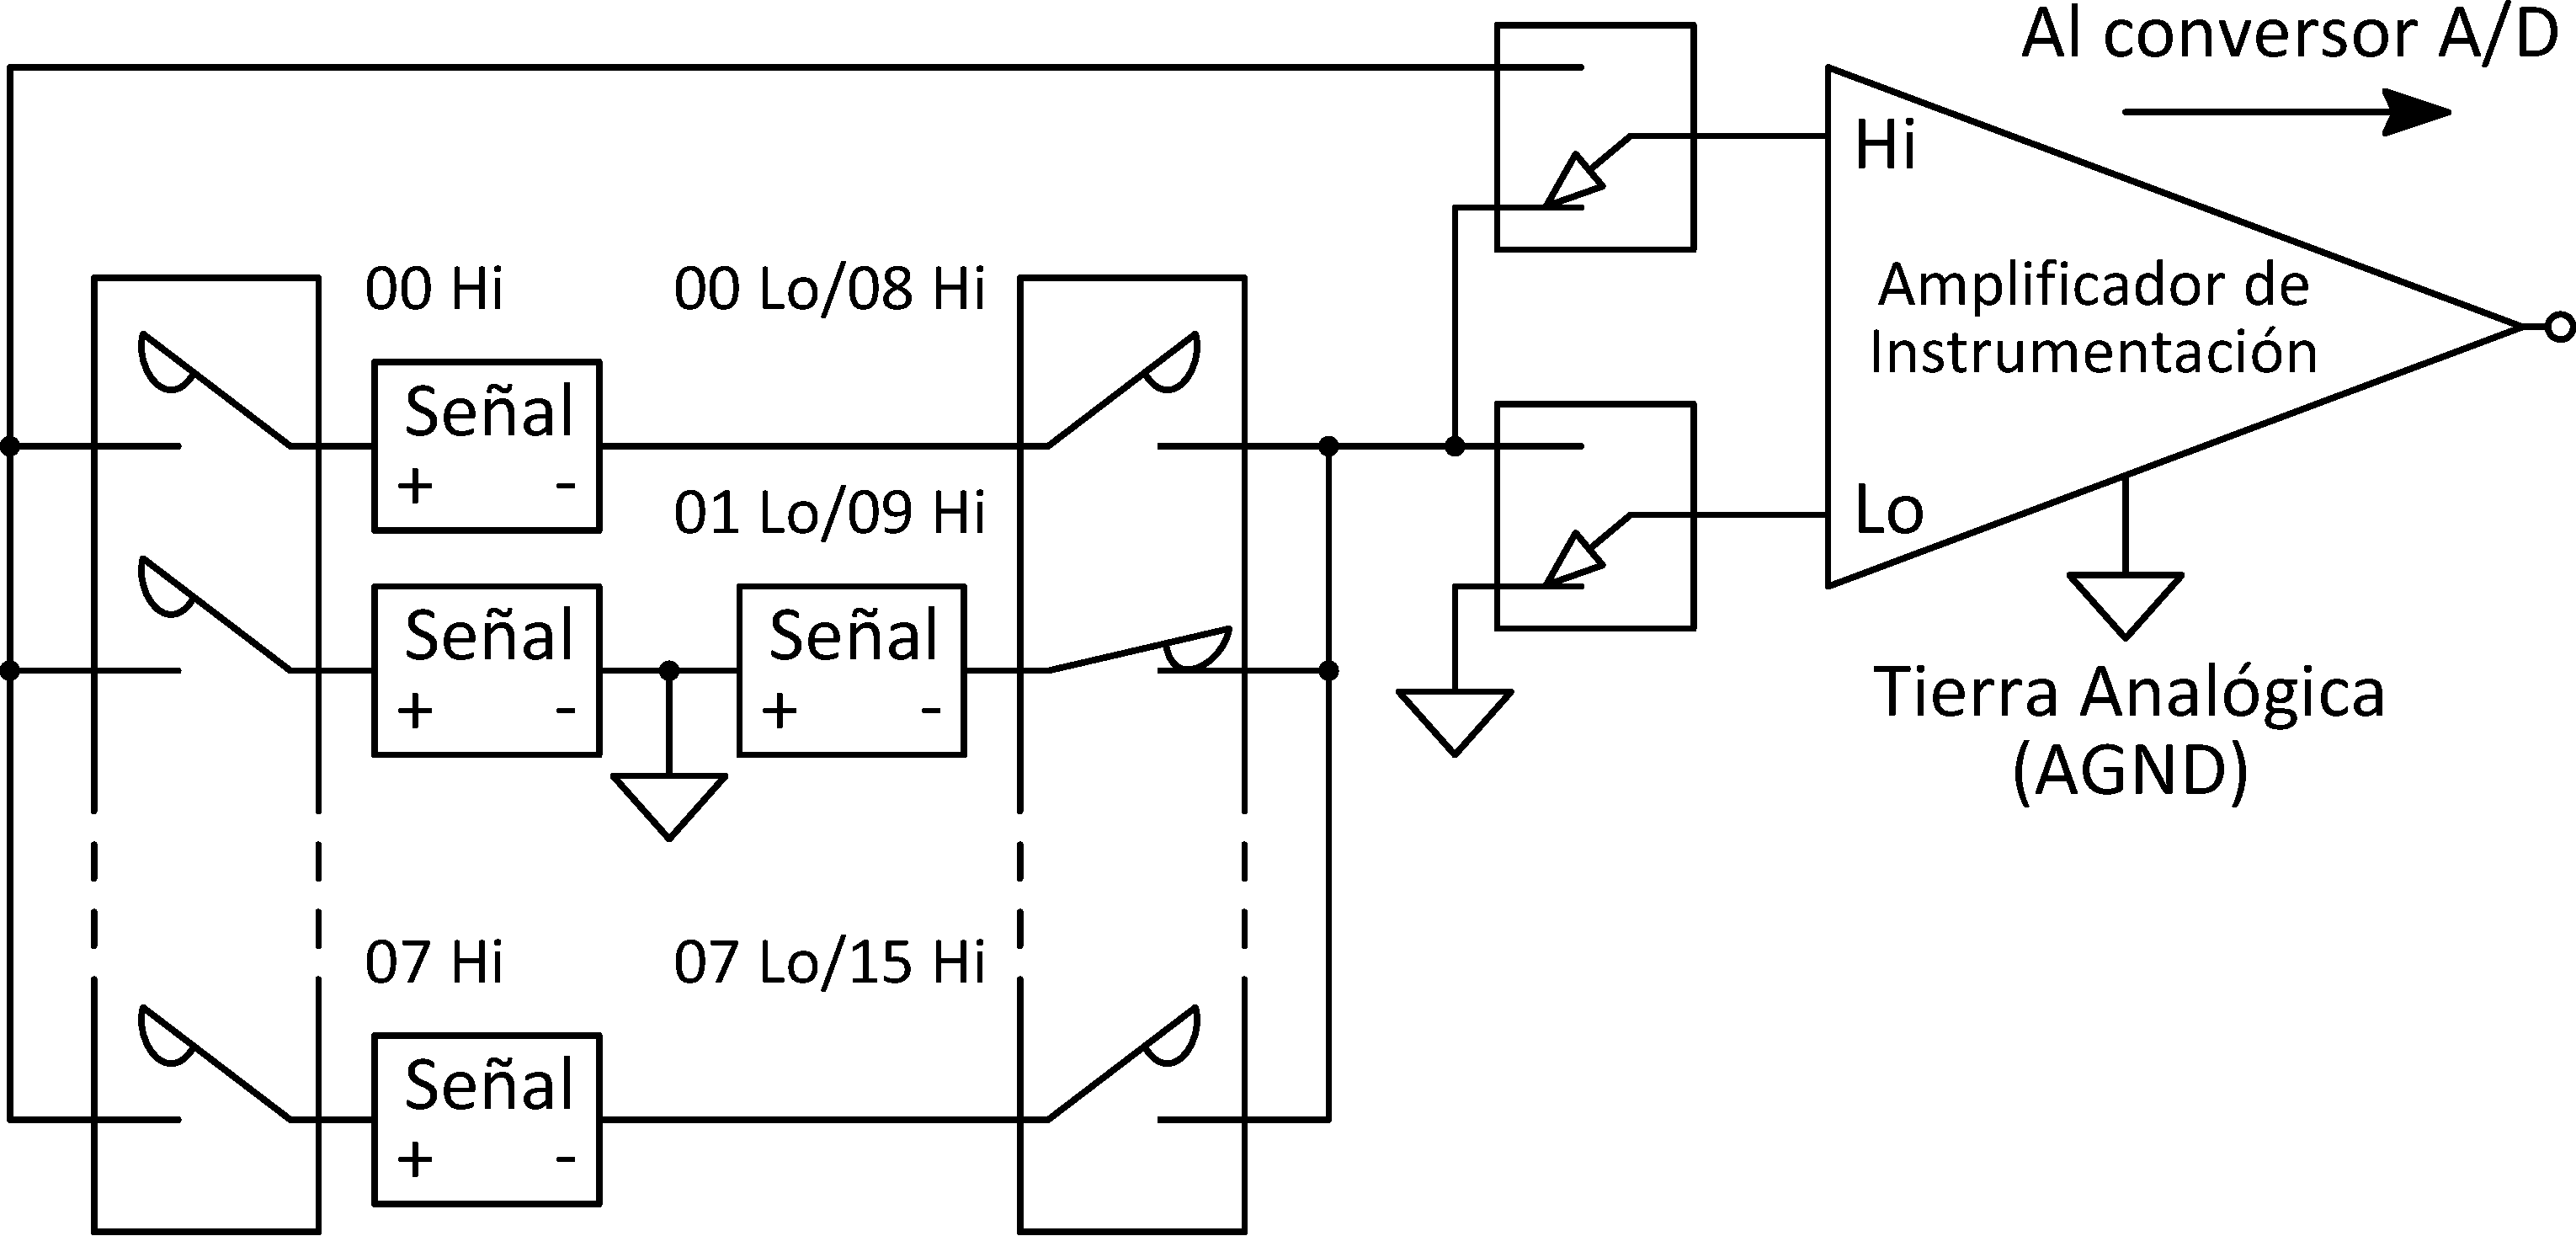
\includegraphics{chapter01-01.pdf}
	\end{center}
	\caption{Figura que muestra el modo de terminaci�n sencillo. La entrada superior del amplificador de instrumentaci�n se conecta al puerto 9 y la entrada inferior se conecta a masa}
	\label{fig:termination-modes}
\end{figure}

Para hacerlo, cabr�a pensar que es suficiente con modificar el atributo que controla el modo de terminaci�n del canal correspondiente. Al contrario de lo que pudiera parecer, el modo de terminaci�n es una propiedad que no es atribuible al canal, si no que se atribuye a un par de puertos\footnote{Aunque seg�n las especificaciones del fabricante es posible configurar cada par de puertos para que opere seg�n un modo de terminaci�n independiente del resto, \matlab{} s�lo admite un modo de terminaci�n para el conjunto total de puertos.}. En concreto, el modo de terminaci�n afecta a los pares de puertos compuestos por un primero de entre los puertos 0 y 7, y un segundo cuyo n�mero de puerto es igual al del primero m�s 8. De ah� que todos los canales relacionados con el mismo par de puertos deban estar configurados con el mismo modo de terminaci�n, una configuraci�n distinta no est� permitida.\par
Los dos modos de terminaci�n posibles se conocen como: diferencial, si es que la se�al que entra en cada terminal del amplificador procede de cada uno de los puertos del par; sencillo, en caso de que uno de los terminales de entrada del amplificador se conecte a la referencia de tensi�n. En este documento se llama canal diferencial a los canales cuyo modo de terminaci�n sea diferencial, y canal con un s�lo terminal o monoterminal a aquellos para los que el modo de terminaci�n es sencillo. \par
Las ventajas que presenta el uso de uno u otro tipo de canales son comprensibles. Emplear canales con un s�lo terminal permite aplicar el proceso de adquisici�n sobre un mayor n�mero de se�ales simult�neamente. Por el contrario, utilizar canales diferenciales redunda en una mayor inmunidad frente al ruido. Adem�s, los amplificadores diferenciales eliminan de forma inherente la componente en continua.\par
\par


\subsection{Rendimiento}\label{subsec:throughput}

Se entiende como rendimiento la cantidad m�xima de operaciones de conversi�n que el dispositivo puede realizar por unidad de tiempo. Para que una de estas operaciones contribuya a la medida de rendimiento debe superar un requisito de precisi�n.\par
El rendimiento �ptimo de la tarjeta \kpci{} especificado por el fabricante es de cien mil operaciones por segundo (100 KS/s). No obstante se advierte, para obtener este nivel de rendimiento es necesario alimentar la tarjeta con una fuente de tensi�n ideal. Adem�s, es importante que exista adaptaci�n de impedancias entre el circuito de alimentaci�n y el puerto por el que se quiere introducir la se�al. A�n en estas condiciones el valor proporcionado por la casa Keithley est� sujeto a un error relativo m�ximo del $0.02\%$, el cual supone un error absoluto m�ximo de dos mil operaciones por segundo (2 KS/s).


\subsubsection[Factores limitantes del rendimiento]{Amplificador de instrumentaci�n y p�rdida del rendimiento}

El amplificador de instrumentaci�n interno de la \kpci{} es de ganancia variable. Es posible configurar una ganancia distinta para cada canal. El prop�sito del amplificador es permitir al usuario modificar la amplitud de la se�al que entra al conversor. La intenci�n que se persigue es conseguir que la conversi�n se enfoque en los detalles de la se�al que sean de mayor inter�s y se pierda la m�nima informaci�n posible. Todo ello a�n trabajando simult�neamente con m�ltiples se�ales cuyo rango de amplitudes es con frecuencia muy diferente.\par
La desventaja que presenta esta configuraci�n ---multiplexor -- amplificador de instrumentaci�n -- conversor--- es una p�rdida de rendimiento que se produce en situaciones determinadas a causa de la intervenci�n del amplificador en la operaci�n de adquisici�n.\par
Cada ciclo de reloj cambia el canal activo y debe cambiar, si es oportuno, la se�al que accede al amplificador. Este proceso no es inmediato. Tras conmutar el multiplexor que precede al amplificador, se da paso al puerto conveniente. No obstante, la se�al que recibe el amplificador presenta, hasta transcurrido un determinado periodo de tiempo, una componente residual de la se�al que se amplific� en el anterior ciclo de reloj. Transcurrido dicho periodo de tiempo la se�al que entra al amplificador se ve libre de esa componente residual y se corresponde �nicamente con la se�al que entrega el multiplexor, se dice que se ha fijado la se�al.\par
Y es as� como el amplificador es causa de p�rdida de rendimiento, por medio de las componentes residuales. Si la conversi�n se realiza antes de fijar la se�al, el conversor toma un valor de la se�al corrompido por la componente residual de la se�al precedente. Por tanto, la muestra resultante queda igualmente corrompida incluso hasta el punto de perder su validez. Las operaciones de conversi�n que tengan como resultado muestras inv�lidas s�lo contribuyen a falsear la medida de rendimiento, haciendo que parezca mayor de lo que en realidad es.\par
El fabricante da a entender que existe una soluci�n de dise�o que resuelve en parte el problema planteado por las componentes residuales. Esta soluci�n consiste en alargar de forma deliberada la duraci�n del ciclo de reloj, de esa forma se proporciona tiempo suficiente para fijar la se�al. Sin embargo, esta soluci�n presenta dos inconvenientes: no solventa el problema en la totalidad de los casos y es, asimismo, una forma de perder rendimiento. Lo cual conduce inevitablemente a una soluci�n de compromiso, alargar el ciclo de reloj lo suficiente para que en la mayor�a de los casos el efecto de las componentes residuales sobre la precisi�n de la conversi�n no invalide las muestras resultantes y se produzca, por tanto, una ca�da del rendimiento, sin que la duraci�n del nuevo ciclo contribuya por s� misma a una p�rdida notable de �ste.\par


\subsubsection{Optimizaci�n del rendimiento}

Como se ha visto, la inclusi�n del amplificador en el dise�o de la tarjeta es causa directa o indirecta de una p�rdida de rendimiento. La magnitud de esa ca�da en el rendimiento depende de la configuraci�n de la cola de muestreo y de la amplitud de la se�al una vez llega �sta al dispositivo de adquisici�n.

\begin{itemize}
	\item Las se�ales cuya tensi�n absoluta se encuentra por debajo de los 100 mV al llegar a la \kpci{} sufren en mayor medida las consecuencias del empleo de un amplificador en la operaci�n de conversi�n. En primer lugar la se�al tarda m�s en fijarse de modo que el rendimiento se reduce a la mitad en las mejores condiciones, de 100 KS/s pasa a 50 KS/s. Esto es debido a que, al ser la amplitud de la se�al y la del ruido comparables, especialmente despu�s de que �ste se vea reforzado por el efecto de las componentes residuales, se genera una mayor incertidumbre.\par
	Por otro lado las se�ales que requieren que el amplificador opere con alta ganancia son las m�s perjudicadas por los problemas que causa el amplificador en configuraciones multiganancia, tal y como se explica a continuaci�n.
	\item Por lo general, el rendimiento se ve afectado de forma m�s pronunciada por el efecto de las componentes residuales en configuraciones multiganancia en las que se encadenan secuencias de canales con ganancia diferente. Una configuraci�n multiganancia de la cola de muestreo implica que en diferentes ciclos de reloj el amplificador act�a con ganancias distintas. Eso con frecuencia significa que el rango en el que se encuentra comprendida la amplitud de las se�ales que est�n entrando al dispositivo de adquisici�n es diferente de una se�al a otra. Cuando as� ocurre puede sucederse en ocasiones que en ciclos de reloj consecutivos entren al amplificador dos se�ales de amplitud diferente, siendo la amplitud de la se�al que ocupa el primer ciclo mucho mayor que la de la otra se�al en el tiempo en el que ambas permanecen a la entrada del dispositivo. Por otro lado, parece l�gico considerar que la componente residual asociada a una se�al cuya amplitud sea predominantemente mayor que la de otra se�al es de mayor amplitud inicial y mayor duraci�n temporal que la asociada a la segunda se�al. Por tanto si ocurre como se ha dicho y se tiene en cuenta la base probable que se ha propuesto, cuando la segunda de las se�ales se convierte en la se�al activa la amplitud de la componente residual asociada a la primera de ellas puede ser suficiente, incluso, para enmascararla.\par No s�lo eso, la amplitud de la se�al que llega m�s tarde al amplificador puede ser, en t�rminos absolutos, la mayor parte del tiempo, menor que la de la otra se�al, al ser as� lo m�s probable es que se amplifique empleando un mayor factor de ganancia. De ser as�, la amplitud de la componente residual a la que se enfrenta esta se�al puede provocar en el peor de los casos que el conversor sature y la p�rdida de precisi�n sea mucho mayor. Sea cual sea el caso, es posible observar entonces, que en configuraciones multiganancia las muestras resultantes se obtienen de una conversi�n menos precisa, en especial si se trabaja con se�ales de peque�a amplitud ---tal y como se especific� en el punto anterior--- o si las ganancias configuradas en la cola de muestreo difieren mucho unas de otras. Aplicando la relaci�n entre la validez de las muestras y el rendimiento de la que se habl� anteriormente, la consecuencia de emplear configuraciones multiganancia es una mayor p�rdida de rendimiento.
	\item En configuraciones monoganancia el uso del amplificador supone una causa indirecta de la ca�da de rendimiento. El dise�o del dispositivo de adquisici�n est� pensado primordialmente para su uso en configuraciones multiganancia, de lo contrario la inclusi�n de un amplificador de ganancia variable en el esquem�tico de la tarjeta ser�a incomprensible. Por la misma raz�n, Keithley adopta una soluci�n de dise�o como la expuesta en el anterior apartado, para tratar de obtener un rendimiento �ptimo en configuraciones multiganancia. Sin embargo, el efecto de las componentes residuales en configuraciones monoganancia es m�nimo y la consecuente p�rdida de rendimiento tambi�n lo es. Por tanto, una soluci�n que consiste en alargar el ciclo de reloj resulta, en configuraciones monoganancia, innecesaria y perjudicial para el rendimiento.
\end{itemize}

Las acciones que el fabricante adopta para tratar de que el usuario obtenga el mayor rendimiento posible del dispositivo no se limitan a aplicar una soluci�n de compromiso en el dise�o de la duraci�n del ciclo de reloj. En el manual de usuario se hacen una serie de recomendaciones de uso orientadas a conseguir este fin.\par
Se proponen varias soluciones, la m�s trivial de las cuales pasa por preamplificar todas las se�ales que vayan a ser objeto del proceso de adquisici�n efectuado por la tarjeta consiguiendo que su amplitud var�e en un mismo rango. Si se hace as�, es suficiente con emplear una configuraci�n monoganancia para minimizar los efectos de las componentes residuales en el rendimiento. Adem�s al preamplificar las se�ales, �stas presentan una mejor relaci�n se�al a ruido, es decir, son menos vulnerables al ruido. Aunque buena, esta soluci�n no deja de ser trivial puesto que el amplificador de instrumentaci�n de la tarjeta pierde toda funcionalidad y pasa a ser un estorbo en el proceso de adquisici�n.\par
La soluci�n de car�cter pr�ctico propuesta por Keithley radica configurar la cola de muestreo de forma <<sensata>>. Como se ha visto, en determinadas ocasiones una configuraci�n inapropiada de la cola de muestreo puede inducir que la p�rdida de rendimiento que provoca la inclusi�n del amplificador en el circuito de adquisici�n sea todav�a mayor. Para evitar que esto ocurra y sacar el m�ximo partido del dispositivo se dan en el manual dos condiciones que de cumplirse garantizan que la cola se encuentre configurada de forma �ptima en t�rminos de rendimiento.

\begin{itemize}
	\item La primera consiste en agrupar canales con distinta ganancia en posiciones consecutivas de la cola, a�n si al hacerlo se pierde el orden de muestreo definido en una primera instancia por el usuario. Si como se presupuso en el apartado anterior, com�nmente dos se�ales que requieren ser amplificadas con el mismo factor de ganancia var�an en el mismo rango de amplitudes, en estas secuencias monoganancia las consecuencias de las componentes residuales en la precisi�n de la conversi�n son m�nimas.
	\item A pesar de emplear una configuraci�n como la anterior, la aparici�n de saltos de ganancia en la cola de muestreo es todav�a probable. Por ejemplo, en la transici�n entre dos secuencias monoganancia como las descritas arriba. El salto es a�n m�s problem�tico si la transici�n se realiza para dar paso a una secuencia de ganancia mayor. El primer canal de esta secuencia sufre en mayor proporci�n los efectos de las componentes residuales y el rendimiento asociado al canal se ve reducido dram�ticamente. Para minimizar el impacto que en determinados canales como �ste tienen los problemas causados por el amplificador, es posible modificar la configuraci�n de la cola para que dichos canales ocupen varias posiciones consecutivas. Esta segunda condici�n persigue dar m�s tiempo para que se fije la se�al cuando los mencionados canales est�n activos. Para ello se necesitan posiciones vac�as en la cola, posiciones que es posible obtener desalojando canales previamente configurados.
\end{itemize}


\section{Comunicaci�n con el perif�rico}

Para la interacci�n con dispositivos externos, la \kpci{} dispone de dos conectores formato mini-\textsc{d} de 36 terminales que cumplen con el est�ndar \textsc{ieee} 1284 de protocolos de comunicaci�n en paralelo. Si se observa la tarjeta como el rect�ngulo que forma desde un punto de vista geom�trico y observ�ndola de frente, los conectores quedan ubicados en un lado de la tarjeta contiguo a aquel en el que se sit�a la conexi�n \textsc{pci}. Todo ello de forma que tras el montaje del perif�rico en la placa base los conectores quedan expuestos en la parte posterior de la carcasa en la que providencialmente debe encontrarse instalada dicha placa, tal y como es habitual en este tipo de dispositivos.\par
En las figuras expuestas a continuaci�n se etiqueta cada terminal seg�n su ubicaci�n relativa con respecto al conector y al resto de terminales en el mismo, para cada conector, mostrando la distribuci�n definida por el fabricante. Las tablas describen el prop�sito de cada terminal y se especifica que tipo de se�al debe circular por los mismos. % Las tablas y figuras dispuestas (disposici�n)

\newsavebox{\auxbox}
\sbox{\auxbox}{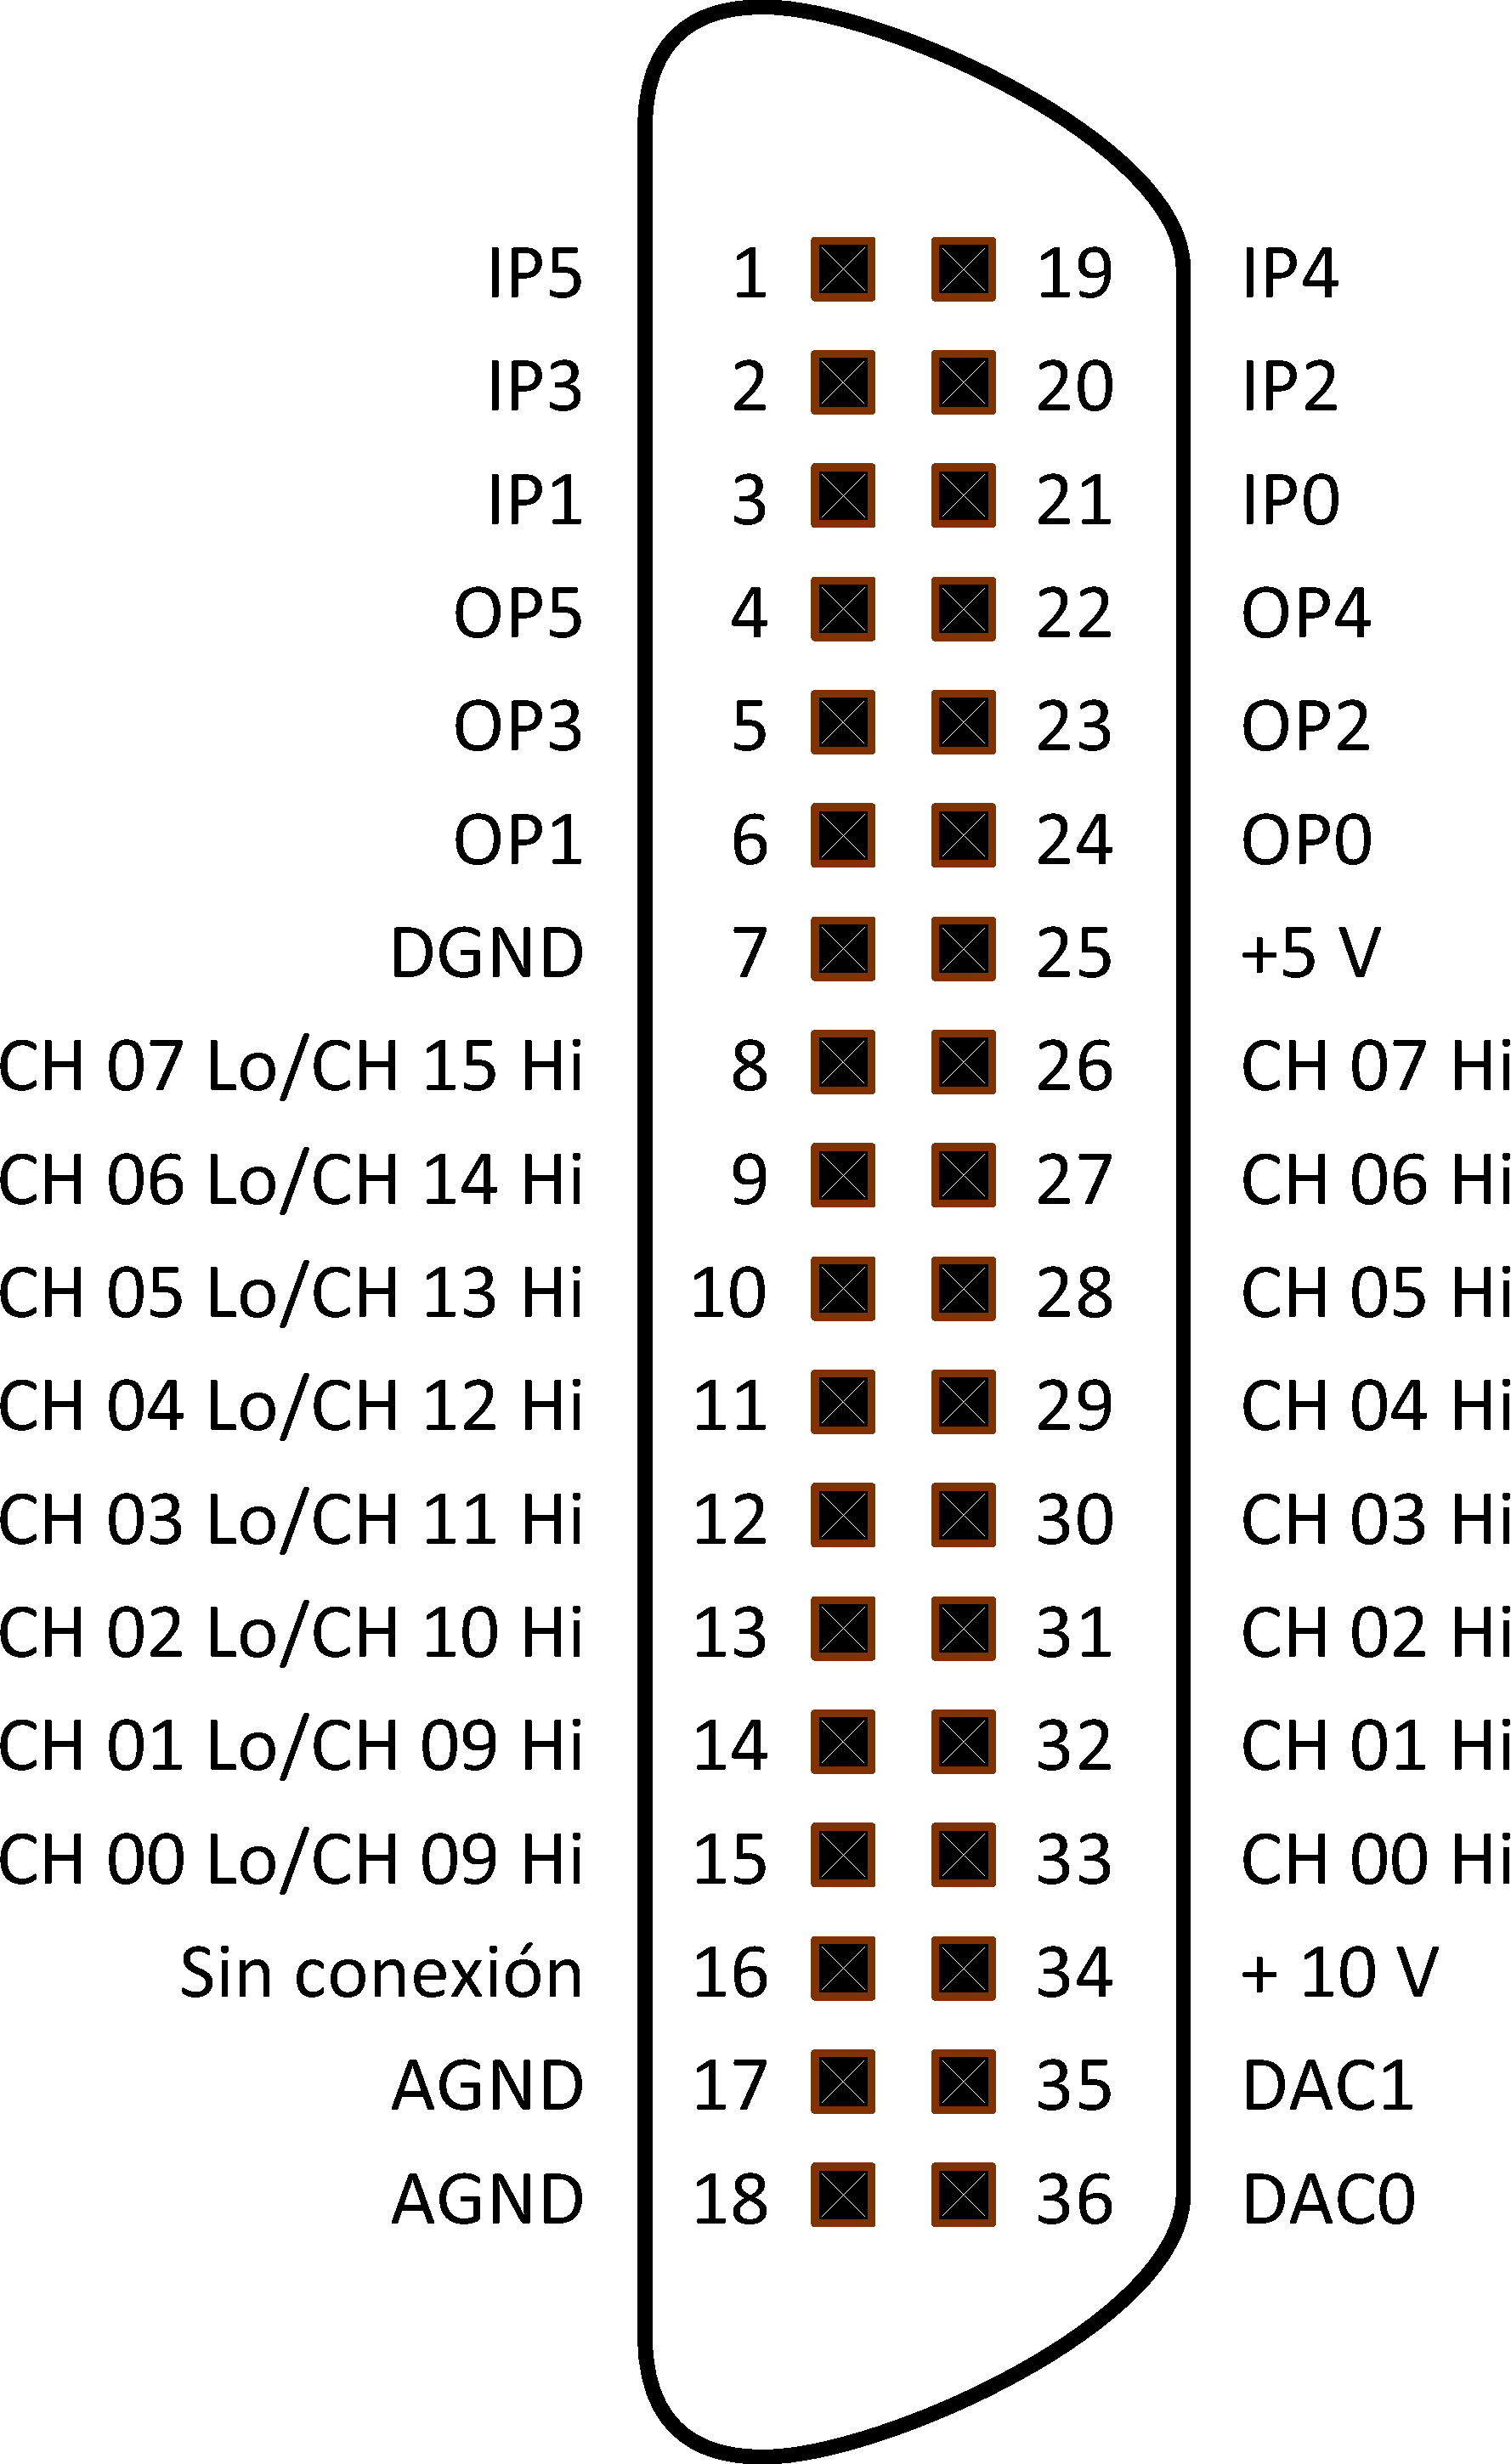
\includegraphics[height=.3\textheight, keepaspectratio=true, angle=90]{chapter01-02.pdf}}
\newlength{\auxheight}
\setlength{\auxheight}{\ht\auxbox + 5pt}
\newlength{\auxwidth}
\setlength{\auxwidth}{\wd\auxbox - 5pt}

\begin{figure}[htbp]
	\centering
	\subfloat[Conector etiquetado como ``analog'']{\vbox  to \auxheight{ %
		\hbox to \auxwidth{
			\hspace*{-7pt}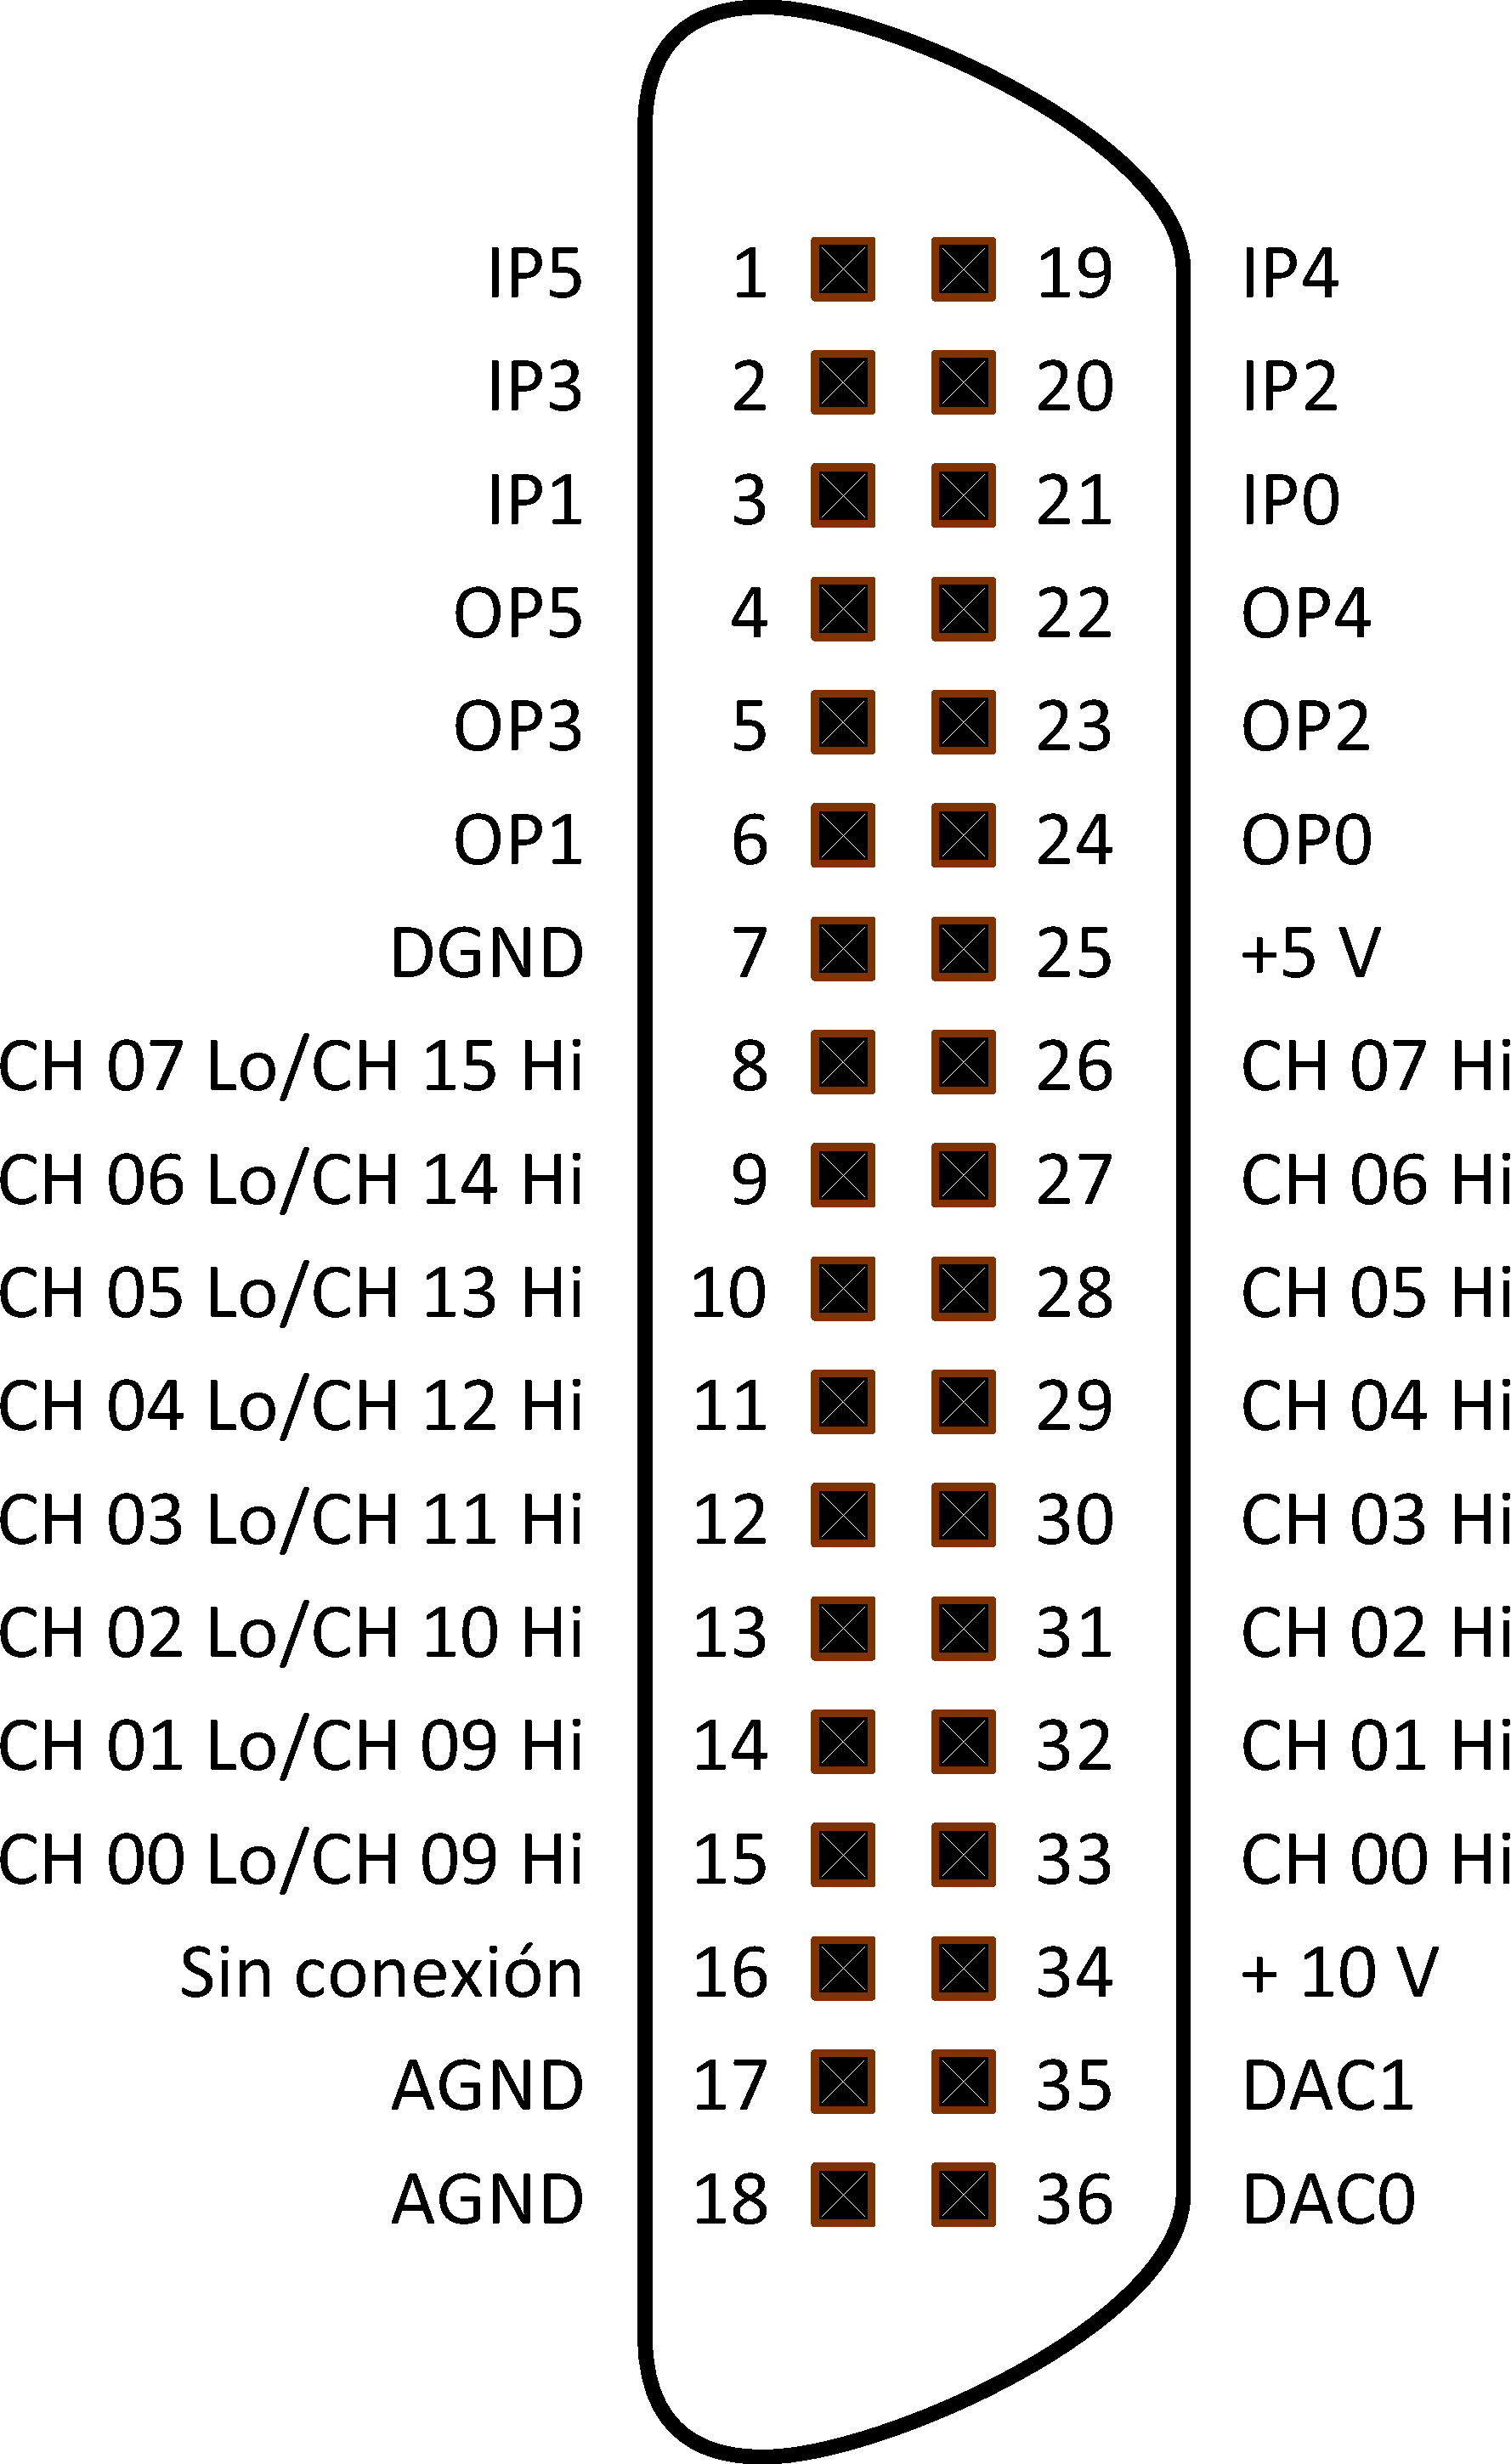
\includegraphics[height=.3\textheight, keepaspectratio=true, angle=90]{chapter01-02.pdf}} %
	\vfil}}\qquad
	\subfloat[Conector etiquetado como ``digital'']{\vbox to \auxheight{\vfil %
		\hbox to \auxwidth{
			\hspace*{-7pt}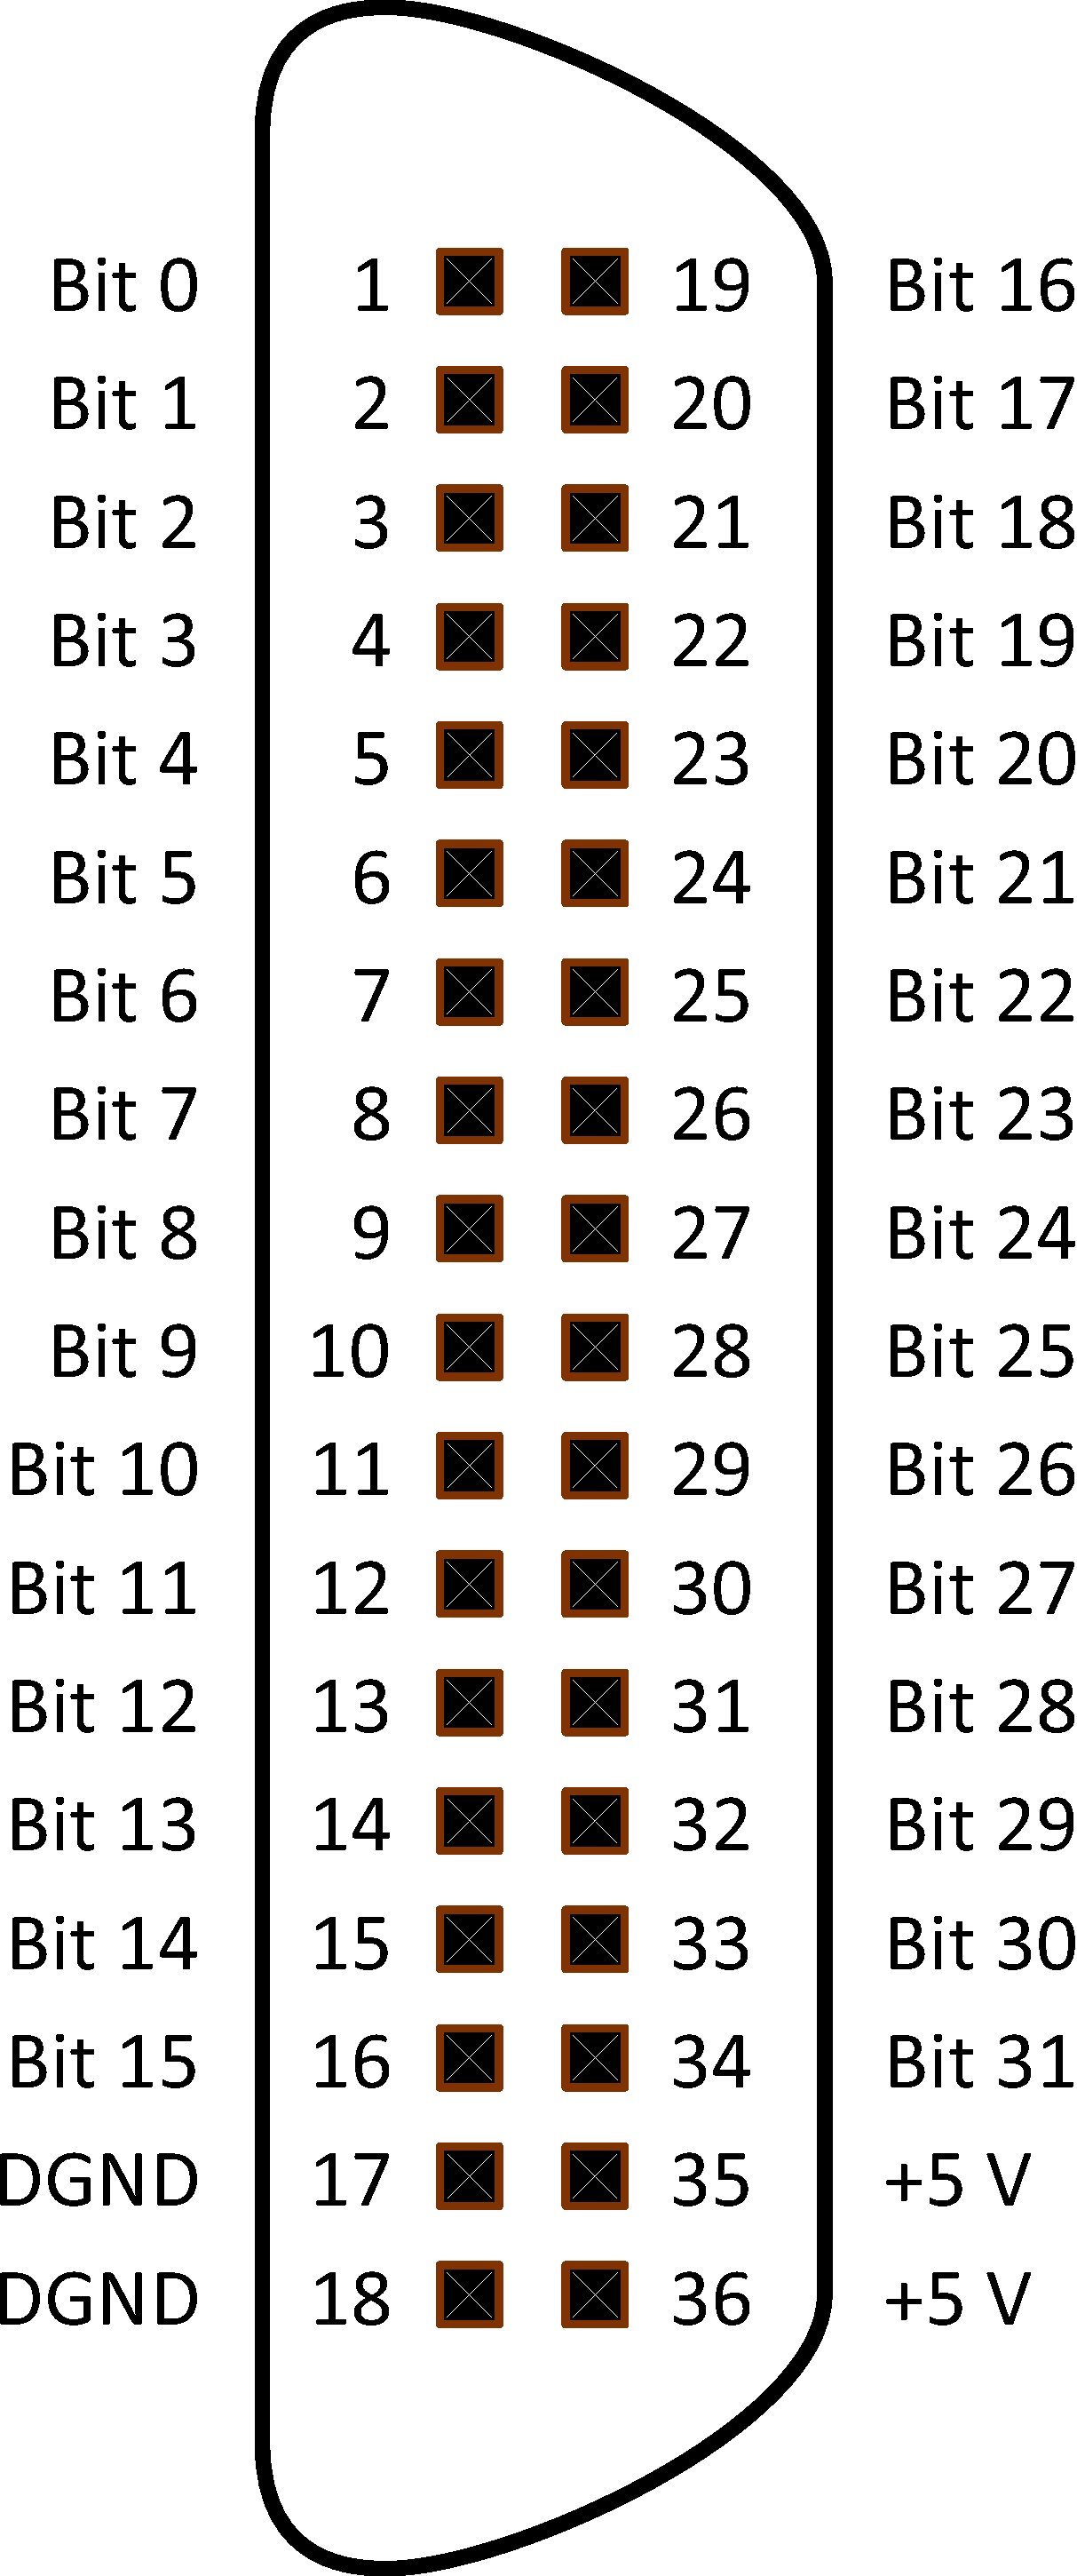
\includegraphics[height=.3\textheight, keepaspectratio=true, angle=90]{chapter01-03.pdf}} %
	\vfil}}
 	\caption{Esquema del panel de conexiones trasero de la \kpci{}}
	\label{fig:ports}
\end{figure}

\begin{table}[p]
	\centering
	\begin{tabular}{>{\raggedleft}p{1cm} >{\scshape}c >{\arraybackslash}l}
		\toprule
		\multicolumn{1}{c}{Terminal} & {\upshape Puerto asignado} & \multicolumn{1}{c}{Descripci�n} \\
		\midrule
		1 & ip5 & \multirow{12}{0.6\textwidth}{Bits digitales de entrada multifunci�n. Pueden ser configurados por el usuario para que ejerzan la funci�n de:\miniit{\item Base temporal para el contador/temporizador y/o entrada a \emph{gate} \\\item Reloj externo para conversiones A/D o D/A \\\item Disparador digital externo \\\item Entrada digital en el modo \emph{target-mode}}} \\
		2 & ip3 & \\
		3 & ip1 & \\
		\\\\\\\\\\\\\\\\
		\midrule
		4 & op5 & \multirow{12}{0.6\textwidth}{Bits digitales de salida multifunci�n. Pueden ser configurados por el usuario para que ejerzan la funci�n de:\miniit{\item Salidas del contador/temporizador\\\item Salida del disparador\\\item Salida de control para accesorios\\\item Salida del reloj interno\\\item Salida digital en el modo \emph{target-mode}}} \\
		5 & op3 & \\
		6 & op1 & \\
		\\\\\\\\\\\\\\\\
		\midrule
		7 & dgnd & \multicolumn{1}{c}{Tierra digital} \\
		\midrule
		8 & ch07 lo/ch15 & \multirow{4}{0.6\textwidth}{Entradas anal�gicas, cuya funci�n depende del modo de terminaci�n configurado: puerto asociado a un canal monoterminal o puerto bajo de un canal diferencial} \\
		9 & ch06 lo/ch14 & \\
		10 & ch05 lo/ch13 & \\
		$\vdots$ & $\vdots$ & \\
		15 & ch00 lo/ch08 & \\
		\midrule
		16 & {\upshape Sin conexi�n} & \\
		\midrule
		\multicolumn{1}{l}{17, 18} & agnd & Tierra anal�gica \\
		\bottomrule
	\end{tabular}
	\caption{Relaci�n entre los puertos y terminales que presenta el conector trasero de la \kpci{} etiquetado como \emph{analog}}
	\label{tab:analog-ports}
\end{table}

\begin{table}[p]\ContinuedFloat
	\centering
	\begin{tabular}{>{\raggedleft}p{1cm} >{\scshape}c >{\arraybackslash}l}
		\toprule
		\multicolumn{1}{c}{Terminal} & {\upshape Puerto asignado} & \multicolumn{1}{c}{Descripci�n} \\
		\midrule
		19 & ip4 & \multirow{12}{0.6\textwidth}{Bits digitales de entrada multifunci�n. Pueden ser configurados por el usuario para que ejerzan la funci�n de:\miniit{\item Base temporal para el contador/temporizador y/o entrada a \emph{gate} \\\item Reloj externo para conversiones A/D o D/A \\\item Disparador digital externo \\\item Entrada digital en el modo \emph{target-mode}}} \\
		20 & ip2 & \\
		21 & ip0 & \\
		\\\\\\\\\\\\\\\\
		\midrule
		22 & op4 & \multirow{12}{0.6\textwidth}{Bits digitales de salida multifunci�n. Pueden ser configurados por el usuario para que ejerzan la funci�n de:\miniit{\item Salidas del contador/temporizador\\\item Salida del disparador\\\item Salida de control para accesorios\\\item Salida del reloj interno\\\item Salida digital en el modo \emph{target-mode}}} \\
		22 & op2 & \\
		21 & op0 & \\
		\\\\\\\\\\\\\\\\
		\midrule
		25 & {\upshape +5 V} & \multirow{2}{0.6\textwidth}{Referencia de tensi�n de 5 voltios de corriente continua extra�dos del bus \textsc{pci} del ordenador} \\
		& & \\
		\midrule
		26 & ch07 hi & \multirow{3}{0.6\textwidth}{Entradas anal�gicas restantes, en el modo de terminaci�n diferencial representan el puerto alto de un canal diferencial} \\
		27 & ch06 hi & \\
		28 & ch05 hi & \\
		$\vdots$ & $\vdots$ & \\
		33 & ch00 hi & \\
		\midrule
		34 & {\upshape +10 V} & \multirow{6}{.6\textwidth}{Entrada dise�ada para proporcionar al dispositivo una referencia externa de precisi�n de 10 voltios mediante una fuente de alta impedancia de salida (La impedancia de entrada de este puerto es equivalente a una resistencia de 1 K$\Omega$ en serie con la impedancia de entrada de la fuente)} \\
		\\\\\\\\\\
		\bottomrule
	\end{tabular}
	\caption[]{Continuaci�n del \vref{tab:analog-ports}}
\end{table}

\begin{table}[p]\ContinuedFloat
	\centering
	\begin{tabular}{>{\raggedleft}p{1cm} >{\scshape}c >{\arraybackslash}l}
		\toprule
		\multicolumn{1}{c}{Terminal} & {\upshape Puerto asignado} & \multicolumn{1}{c}{Descripci�n} \\
		\midrule
		35 & dac1 & \multirow{2}{.6\textwidth}{Salida n�mero 1 del conversor digital a anal�gico de la \kpci{}} \\
		\\
		\midrule
		36 & dac0 & \multirow{2}{.6\textwidth}{Salida n�mero 0 del conversor digital a anal�gico de la \kpci{}} \\
		\\
		\bottomrule
	\end{tabular}
	\caption[]{Continuaci�n del \vref{tab:analog-ports}}
\end{table}

\begin{table}[p]
	\centering
	\begin{tabular}{>{\raggedleft}p{1cm} >{\scshape}c >{\arraybackslash}l}
		\toprule
		\multicolumn{1}{c}{Terminal} & {\upshape Puerto asignado} & \multicolumn{1}{c}{Descripci�n} \\
		\midrule
		1 & {\upshape Bit 0} & \multirow{6}{0.6\textwidth}{Canal 0 de bits de entrada/salida de prop�sito general (En la \kpci{} los bits digitales se agrupan de en ocho en ocho en canales. Los canales de este tipo puede configurarse para que los bits que lo integran se comporten como todo salidas o todo entradas)} \\
		2 & {\upshape Bit 1} & \\
		3 & {\upshape Bit 2} & \\
		$\vdots$ & $\vdots$ & \\
		8 & {\upshape Bit 7} & \\
		\\
		\midrule
		9 & {\upshape Bit 8} & \multirow{2}{0.6\textwidth}{Canal 1 de bits de entrada/salida de prop�sito general} \\
		10 & {\upshape Bit 9} & \\
		11 & {\upshape Bit 10} & \\
		$\vdots$ & $\vdots$ & \\
		16 & {\upshape Bit 15} & \\
		\midrule
		\multicolumn{1}{l}{17, 18} & dgnd & Tierras digitales \\
		\midrule
		19 & {\upshape Bit 16} & \multirow{2}{0.6\textwidth}{Canal 2 de bits de entrada/salida de prop�sito general} \\
		20 & {\upshape Bit 17} & \\
		21 & {\upshape Bit 18} & \\
		$\vdots$ & $\vdots$ & \\
		26 & {\upshape Bit 23} & \\
		\midrule
		27 & {\upshape Bit 24} & \multirow{2}{0.6\textwidth}{Canal 3 de bits de entrada/salida de prop�sito general} \\
		28 & {\upshape Bit 25} & \\
		29 & {\upshape Bit 26} & \\
		$\vdots$ & $\vdots$ & \\
		34 & {\upshape Bit 31} & \\
		\midrule
		\multicolumn{1}{l}{35, 36} & {\upshape +5 V} & +5 \textsc{vdc} desde el bus del ordenador \\
		\bottomrule
	\end{tabular}
	\caption{Relaci�n entre los puertos y terminales que presenta el conector trasero de la \kpci{} etiquetado como \emph{digital}}
	\label{tab:digital-ports}
\end{table}


\subsection{Desarrollo de una nueva interfaz}\label{subsec:connection-box}

Por razones pr�cticas, la interfaz original de la \kpci{} basada en dos conectores mini-\textsc{d} no se acomoda a las necesidades que se prev� surgir�n durante el desarrollo de las pruebas requeridas para la finalizaci�n de este proyecto de fin de carrera. En consecuencia, con el prop�sito de agilizar en la medida de lo posible la realizaci�n de estos ensayos, se decide ampliar la interfaz existente.\par
Para ello se parte de dos extremos de cable terminados en un conector tipo macho y desprovistos de cubierta, de cada uno de los cuales surgen 36 hilos de cobre recubiertos de pl�stico flexible coloreado. El patr�n de coloreado de las cubiertas individuales es �nico y no se repite en ninguno de los 36 hilos de que se compone cada extremo de cable. A partir de ah�, se identifica cada terminal de cada conector con el hilo de cobre correspondiente, relacionando las etiquetas que el fabricante pone a los terminales con el c�digo de colores de la cubiertas individuales.\par
Una vez recopilada esta informaci�n, se planea la construcci�n de una caja de conexiones. El dise�o de la caja contempla que se equipe �sta con 72 conectores banana hembra soldados a los 72 hilos de cobre y que comunican con los terminales de los conectores mini-\textsc{d} en los que termina el otro extremo de los cables. Adem�s se planifica la inclusi�n de cuatro conectores coaxiales con rosca con conexiones redundantes a las que se presupone son las cuatro puertas cuyo uso ser� m�s frecuente, las correspondientes al primer canal anal�gico diferencial y las tierras anal�gicas; para as� facilitar el uso continuado de las mismas. Por �ltimo se decide etiquetar la caja de conexiones con marbetes que reproduzcan la nomenclatura visible en la \vref{fig:ports}.\par

\begin{figure}[htbp]
	\begin{center}
		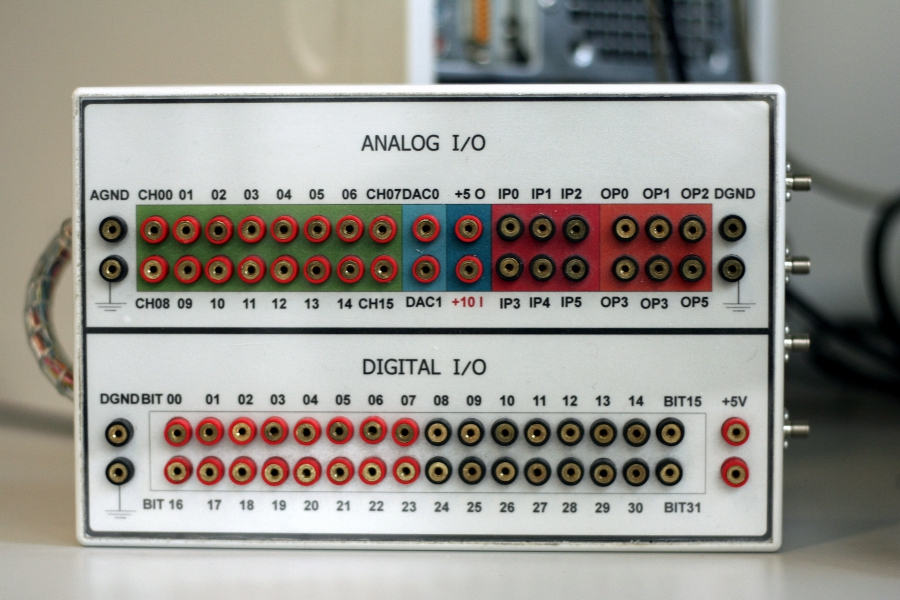
\includegraphics{chapter01-04.jpg}
	\end{center}
	\caption{Plano de la caja de conexiones ya terminada}
	\label{fig:connection-box}
\end{figure}

Puede observarse una representaci�n de la caja de conexiones ya terminada en la \vref{fig:connection-box}. As� mismo se ha a�adido un diagrama que representa dicha caja con mayor claridad.


\chapter{Aplicaci�n para el control de la tarjeta}

\section{Introducci�n}

La consecuencia directa de emplear la \kpci{} como instrumento principal en la adquisici�n de se�ales anal�gicas en contraposici�n con un dispositivo de adquisici�n aut�nomo que no requiera de un \textsc{pc} que lo gobierne, es la necesidad de un software de control que se ocupe entre otras de las siguientes tareas:

\begin{itemize}
	\item Iniciar y detener la sesi�n de adquisici�n.
	\item Interactuar con los drivers de la tarjeta por medio del sistema operativo para controlar por voluntad del usuario par�metros de la sesi�n de adquisici�n como pueden ser, por ejemplo, puertos de entrada, modos de adquisici�n y terminaci�n, o frecuencia de muestreo.
	% \item Realizar el mantenimiento de los buffers de la tarjeta de adquisici�n. Tarea que incluye dar formato a las muestras almacenadas en el o los buffers y trasladar las mismas a la memoria secundaria del \textsc{pc} para que de ese modo puedan ser posteriormente manipuladas.
	\item Realizar el mantenimiento de los buffers de memoria. Tarea que puede dividirse o consta a su vez de dos tareas menores: dar formato a las muestras almacenadas en el o los buffers situados en la memoria interna de la tarjeta para su comprensi�n por parte del ordenador anfitri�n; trasladar las muestras formateadas adecuadamente a la memoria del \textsc{pc} para que de ese modo puedan ser manipuladas por el usuario.
\end{itemize}

La idea original consist�a en dotar al software de control de una interfaz de usuario con la que controlar c�modamente todos estos aspectos de la sesi�n de adquisici�n. A partir de ah� y puesto que ha de hacerse un esfuerzo para desarrollar la aplicaci�n de control se decide dise�ar el software de forma que pueda desarrollar competencias adicionales. As�, adem�s de las tareas b�sicas que corresponden al software de control, se dise�a la aplicaci�n para que pueda cumplir con los siguientes cometidos.

\begin{itemize}
	\item Mostrar en un visor el valor de las muestras resultantes de muestrear la se�al a 4 muestras por segundo.
	\item En un modo de funcionamiento diferente, mostrar en el mismo visor, cada cuarto de segundo aproximadamente, la media aritm�tica del valor de las muestras recogidas en dicho periodo a una frecuencia de muestreo especificada por el usuario.
	\item Funcionando en el modo gr�fico, representar la se�al y el espectro en frecuencia de la misma en dos espacios de coordenadas separados. A voluntad del usuario pueden ser habilitadas o deshabilitadas cualquiera de estas dos representaciones o ambas.
\end{itemize}


\subsection{Funcionamiento de un osciloscopio}

El prop�sito de este segundo cap�tulo es guiar al lector en el proceso de elaboraci�n y prueba del software de control. Como se ha mencionado anteriormente, en el proceso de dise�o previo a la programaci�n del software se decide incluir en la aplicaci�n un modo de funcionamiento que permita representar la forma de la se�al y su espectro en frecuencia. Una parte importante del c�digo fuente del software de control lo ocupan las rutinas con las que se implementa dicho modo de funcionamiento. Adem�s, la influencia que ejerce este conjunto de rutinas sobre el resto es notable. De hecho, del resto de funciones, muchas se han escrito a partir de �ste n�cleo de c�digo, acomod�ndose a �l.\par
Muchas de las ideas que han resultado ser imprescindibles para llevar a t�rmino el proceso de desarrollo del software se han obtenido tras observar el comportamiento de un osciloscopio de laboratorio. Una serie de conceptos que han influido en la forma y estructura del c�digo fuente final. La elecci�n de un osciloscopio digital como modelo es intencionada ya que desde un principio lo que se persigue es obtener unas prestaciones similares, prestaciones que se observan en el resultado final (v�ase el ap�ndice \vref{chap:apendixA}).\par
Por todo ello, para comprender como se ha ido desarrollando el software, para entender como funciona la aplicaci�n de usuario, es conveniente conocer las claves que se siguieron durante el curso de su desarrollo, en definitiva, las pautas de comportamiento de un osciloscopio. De una forma resumida se expone aqu� un texto en relaci�n con dicha materia para que el lector pueda llegar a estas conclusiones.


\subsection{Osciloscopios anal�gicos, osciloscopios digitales y retardo}

Los osciloscopios anal�gicos emplean un tubo de rayos cat�dicos y un monitor de f�sforo para generar una imagen de la se�al. El cursor que el tubo dibuja en el monitor lo va barriendo de izquierda a derecha con periodicidad, y su posici�n vertical refleja a cada momento el valor de tensi�n de la se�al el�ctrica que entra al osciloscopio. El monitor preserva durante breves instantes una traza del cursor y as� se forma la imagen que representa a la se�al.\par
En la actualidad suelen emplearse osciloscopios digitales. El procedimiento que sigue un osciloscopio digital para representar se�ales es completamente diferente al que siguen los osciloscopios anal�gicos. No existe ning�n cursor, se generan fotogramas de la se�al en seguimiento\footnote{En realidad, los osciloscopios digitales modernos pueden representar por pantalla varias se�ales simult�neamente.}, im�genes completas que cubren la pantalla entera con un fragmento de se�al, una vez aparece una imagen por pantalla permanece est�tica hasta que una nueva imagen la sustituye. La dimensi�n temporal de la representaci�n determina en teor�a cuanto debe esperar el osciloscopio desde que se muestra por pantalla una imagen hasta que se puede generar la siguiente. La espera resulta evidente puesto que la se�al no se conoce de antemano, al contrario que ocurre con los osciloscopios anal�gicos que representan la se�al en tiempo real, si se desea representar por pantalla un fragmento de la se�al de una determinada duraci�n el osciloscopio debe esperar hasta que transcurra dicho periodo de tiempo. En otras palabras, aparece un retardo que depende exclusivamente de la duraci�n del fragmento de se�al necesario para cubrir la ventana del osciloscopio, o lo que es lo mismo, el retardo es independiente de otros par�metros como son la velocidad de muestreo o la potencia de procesado del osciloscopio.\par
Este modo de proceder tiene un inconveniente, el objetivo de un osciloscopio es mostrar en cada momento como es la forma de la se�al, si el retardo introducido es demasiado alto el osciloscopio deja de ser eficaz pues la informaci�n que proporciona cada imagen es obsoleta. Problema que se ve agravado por la posibilidad de configurar el eje de tiempos. As� es, tanto los osciloscopios anal�gicos (variando la frecuencia de barrido del cursor) como los osciloscopios digitales, permiten que el usuario modifique la cantidad de tiempo que refleja el eje horizontal de la representaci�n, pudiendo ser �sta mayor o menor. A efectos pr�cticos, en los osciloscopios digitales el tiempo abarcado por el eje temporal act�a como el inverso de la frecuencia de refresco del monitor, por tanto, cuanto mayor sea ese tiempo con mayor lentitud se suceder�n las im�genes y habr� un mayor desfase entre la se�al y la representaci�n de �sta.


\subsection{Modos de representaci�n en los osciloscopios digitales}\label{subsec:representation-modes}

Para evitar que en determinadas configuraciones del eje temporal del osciloscopio el retardo sea excesivo, la mayor�a de estos dispositivos implementan dos modos de funcionamiento: el modo convencional que se aplica en situaciones en las que el retardo no se considera importante; y una especie de modo continuo. Existen dos criterios que se siguen de manera habitual para diferenciar en que momento es m�s apropiado el uso de uno u otro modo: % En cierto modo esa es una forma de configurar el retardo o el volumen de im�genes mostradas por segundo en un osciloscopio digital. M�s tiempo transcurrir� entre una imagen y la siguiente. M�s anticuada ser� la informaci�n mostrada por pantalla. En el cual la forma de representar se asemeja a la que se da en osciloscopios anal�gicos.

\begin{itemize}
	\item El primer criterio eval�a el correcto funcionamiento del modo convencional. Como se ver� m�s adelante, el modo convencional de representaci�n en un osciloscopio requiere que la cantidad de im�genes que salen por pantalla cada segundo sea lo suficiente grande como para que se simule el movimiento. Por tanto para satisfacer el primer criterio, la tasa de refresco del monitor del osciloscopio debe superar las veintis�is im�genes por segundo o encontrarse alrededor de esta cifra.
	\item El segundo criterio est� relacionado con la funci�n de disparo que se da en el modo convencional de representaci�n. Para poder efectuar correctamente el disparo sobre se�ales de baja frecuencia, al generar cada imagen el osciloscopio debe haber registrado al menos un ciclo de la se�al pertinente\footnote{En la pr�ctica se necesita algo m�s de un ciclo de una se�al para poder garantizar el correcto disparo de �sta. Sin embargo, es com�n conseguir disparar una se�al aunque la configuraci�n del eje de tiempos del osciloscopio permita s�lo obtener una fracci�n del ciclo completo de esa se�al durante la realizaci�n de cada fotograma.}. Lo cual reduce la tasa m�nima de refresco a la frecuencia de la se�al m�s lenta que se desee representar de forma correcta en el modo convencional de representaci�n del osciloscopio.
\end{itemize}

Como puede verse el segundo criterio es m�s restrictivo pues depende de la frecuencia de la se�al y �sta puede ser en efecto inferior a un hercio, es por ello que se emplea habitualmente. Siendo as�, la tasa de refresco m�nima que se permite en el modo convencional en la gran mayor�a de dispositivos y que se ha adoptado para el software de control, es de cinco im�genes por segundo (5 Hz). Cuando se configura un osciloscopio en el modo convencional para que trabaje a esta tasa de refresco es habitual poder visualizar se�ales de frecuencia cercana a 1 Hz, sin embargo la representaci�n se optimiza para configuraciones en las que el osciloscopio muestra, al menos, veinticinco im�genes por segundo, lo cual es apropiado para se�ales con una frecuencia m�nima de 50 Hz. Si la configuraci�n del eje de tiempos del osciloscopio obligara al dispositivo a trabajar con una frecuencia de refresco inferior a la especificada, autom�ticamente conmuta para funcionar en el modo continuo.


\subsubsection{Representaci�n en modo continuo}

Una vez visto cual es la frecuencia umbral a la que el dispositivo conmuta entre los dos modos, debe explicarse que diferencia un modo de funcionamiento de otro. Para ello se expone a continuaci�n cuales son los fundamentos de uno y otro modo. La representaci�n en \emph{modo continuo} es, por decirlo as�, ininterrumpida. La imagen de la se�al de inter�s se desplaza de derecha izquierda a medida que transcurre el tiempo. Para lograr este efecto se aumenta la frecuencia de refresco a expensas de que, como es sabido, el fragmento de se�al obtenido para cada imagen no cubrir� la pantalla al completo. Ocurre as� por que la frecuencia de refresco es muy alta para el eje temporal que representa una gran cantidad de tiempo, por tanto, entre dos im�genes no transcurre el tiempo abarcado por la dimensi�n horizontal de la representaci�n. La primera imagen sit�a el fragmento de se�al que se ha digitalizado en el extremo derecho de la representaci�n, el resto se deja en blanco. Con cada nueva imagen se desplaza el fragmento de se�al representado hasta el momento el suficiente espacio hacia la izquierda como para incorporar un nuevo fragmento de se�al. As� la porci�n de se�al representada aumenta cada vez m�s hasta que el extremo izquierdo de la figura alcanza el margen izquierdo de la ventana del osciloscopio. Cuando esto ocurre, empieza un desplazamiento c�clico, al incorporar un nuevo fragmento de se�al a la derecha se retira un fragmento de la misma proporci�n temporal al otro extremo. La alta tasa con la que aparecen las im�genes por pantalla garantizan que la representaci�n siga casi en tiempo real ---por lo menos as� lo percibe el ojo humano--- a la se�al verdadera. Debe notarse, no obstante, que este m�todo de representaci�n no es adecuado para se�ales de alta frecuencia pues aunque el eje temporal abarque un tiempo mayor, la dimensi�n del monitor obviamente no var�a y las se�ales de alta frecuencia aparecer�n en exceso comprimidas.\par


\subsubsection{Representaci�n en modo convencional}

El \emph{modo convencional} de representaci�n es algo m�s complicado. Como se ha declarado con anterioridad en este mismo apartado, la representaci�n convencional basa su funcionamiento en im�genes que muestran fragmentos de se�al que cubren la dimensi�n temporal de la ventana del osciloscopio y que se suceden unas a otras con presteza. La idea que persigue este m�todo es la de conseguir algo semejante a una pel�cula de la se�al. Para ello, no es s�lo suficiente con que aparezcan muchas im�genes por segundo en el monitor del osciloscopio, esas im�genes deben estar de alg�n modo relacionadas entre s�. Si las im�genes que aparecen en el monitor son de forma consecutiva muy diferentes es probable que no pueda discernirse nada claro, y de nada valdr� la representaci�n.\par
Ah� es donde entra en juego el procesado y la funci�n de disparo de un osciloscopio digital. Cuando un fragmento suficientemente largo como para cubrir la ventana de representaci�n se digitaliza y se almacena en memoria, empieza el procesado digital del mismo. El prop�sito del procesado es, ente otras cosas, eliminar las posible componente en continua, averiguar informaci�n adicional de la se�al en la medida de lo posible, como p.e. su valor de pico a pico, o implementar una funci�n de disparo. La funci�n de disparo del osciloscopio persigue alinear los ejes verticales de la ventana donde se representa con los cruces de la se�al con respecto a un determinado valor de umbral que puede ser configurado por el usuario. La idea es alinear al menos el cruce m�s centrado de cada fragmento de se�al con el eje de abscisas que corta en dos mitades la ventana. Para conseguirlo, durante el procesado se detectan todos los cortes de la se�al con el umbral y despu�s se desplaza el fragmento de se�al para que el corte m�s centrado case con el eje de abscisas. Si la se�al es peri�dica las variaciones entre un fotograma y el siguiente ser�n m�nimas, puesto que ambos estar�n alineados, y se simular� con �xito el movimiento.\par
No obstante, la necesidad de desplazar el fragmento de se�al que va a representarse presenta un inconveniente importante. Para poder desplazar el fragmento de se�al y que se cubra completamente la ventana del osciloscopio su duraci�n, la del fragmento de se�al digitalizado, debe ser superior al tiempo reflejado en el eje de tiempos de la ventana. De lo contrario la se�al aparecer� truncada, se mostrar� un espacio en blanco y, con una tasa de refresco alta, la visualizaci�n ser� confusa. Desplazar fragmentos de se�al implica dos cosas: por un lado el osciloscopio debe esperar m�s tiempo para refrescar la pantalla, es decir, se reduce la tasa de refresco para una misma configuraci�n del eje de tiempos; y por otro, al tener para representar un fragmento de se�al de mayor duraci�n que la reflejada por el eje temporal de la ventana parte del fragmento queda ahora fuera de la representaci�n.\par
Este inconveniente se ve paliado por el hecho de que el modo convencional contempla en principio trabajar con se�ales de alta frecuencia. Estas se�ales cambian de forma tan r�pida que de no ser por el disparo ser�a imposible observar los cambios. Por otro lado puede seleccionarse que informaci�n que se muestra por pantalla accionando un control de offset temporal o modificando el valor de umbral de disparo y, generalmente, la p�rdida de informaci�n a causa del disparo no es significativa.
%\vspace*{99pt}


\section{Elaboraci�n del software de control}


\subsection{Elecci�n del entorno de desarrollo}

El lenguaje o, mejor dicho, plataforma que se ha empleado para el desarrollo del software de control es \matlab{}, la raz�n, su inmejorable compatibilidad con el hardware disponible. A partir de ah�, los componentes de \matlab{} que se han empleado para conseguir que el software de control gozase de las caracter�sticas previstas en la etapa de dise�o son dos: el entorno de desarrollo de interfaces gr�ficas de usuario (\textsc{gui}) de \matlab{}, m�s conocido como \textsc{guide} (\emph{graphical user interface development environment}); y el \datx{} de \matlab{}. El primero de ellos se ha empleado para, como su nombre indica, crear la interfaz que comunica el dispositivo con el usuario. Esta comunicaci�n se hace a trav�s del segundo de los componentes mencionados, �ste permite, mediante comandos de \matlab{} que pueden incluirse en rutinas o llamarse por separado, manejar el dispositivo ---convocarlo a muestrear, configurar sus propiedades--- y administra autom�ticamente los resultados almacen�ndolos en b�ffers situados en la memoria vol�til del ordenador, haci�ndolos de este modo accesibles al administrador de la tarjeta.


\subsection{Data Acquisition Toolbox}

La pr�ctica de emplear \textsc{gui}s como fondo para aplicaciones desarrolladas con \matlab{} es bastante habitual, as� como lo es programar esas interfaces mediante \textsc{guide}. Por ello, y dado que la documentaci�n que se ci�e a tratar la problem�tica que envuelve esta actividad es abundante, se ha preferido dejar a cargo de dichos documentos este asunto y centrar este escrito en presentar con concisi�n los principios necesarios para emplear con �xito la \datx{} de \matlab{} en el manejo de dispositivos para la adquisici�n de se�ales anal�gicas. La f�rmula elegida con tal prop�sito consiste en describir cual es el procedimiento habitual en una sesi�n de adquisici�n de datos y en cada paso detallar las opciones m�s significativas y proporcionar ejemplos explicativos extra�dos del mismo c�digo que integra el software de control.\par
En cuanto a la documentaci�n adicional que el lector puede consultar a continuaci�n se citan varios documentos clasificados en funci�n del tema que tratan. Para la programaci�n de \textsc{gui}s con \matlab{} puede consultarse el manual de usuario, cite, disponible en la web del fabricante. Esta secci�n se basa en la gu�a r�pida sobre el uso de la \datx{}, tambi�n a cargo de \emph{The MathWorks, Inc.}, la compa��a que mantiene la suite matem�tica en cuya web puede obtenerse un documento extendido.


\subsubsection{Componentes de la herramienta}

Los elementos de \matlab{} que juegan un papel suficientemente importante en el funcionamiento de la \datx{} son los listados en el \ref{tab:toolbox-components}.

\begin{table}[htbp]
	\centering
	\begin{tabulary}{.9\textwidth}{C L}
		\toprule
		Componente & \multicolumn{1}{c}{Prop�sito} \\
		\midrule
		Ficheros *.m & Se emplean para automatizar la creaci�n de objetos dispositivo, adquirir datos, configurar las propiedades del dispositivo y la sesi�n, y evaluar el estado de la adquisici�n y los recursos.\\
		\midrule
		M�quina virtual de adquisici�n de datos & Almacena objetos dispositivo y sus propiedades, controla el almacenamiento de los datos adquiridos y controla la sincronizaci�n de eventos.\\
		\midrule
		Adaptadores & Son la v�a de comunicaci�n entre la m�quina virtual de adquisici�n de datos y el hardware por la cual se transmiten propiedades, datos y eventos.\\
		\bottomrule
	\end{tabulary}
	\caption{Descripci�n de los componentes de la \datx{}}
	\label{tab:toolbox-components}
\end{table}

\begin{figure}[htbp]
	\begin{center}
		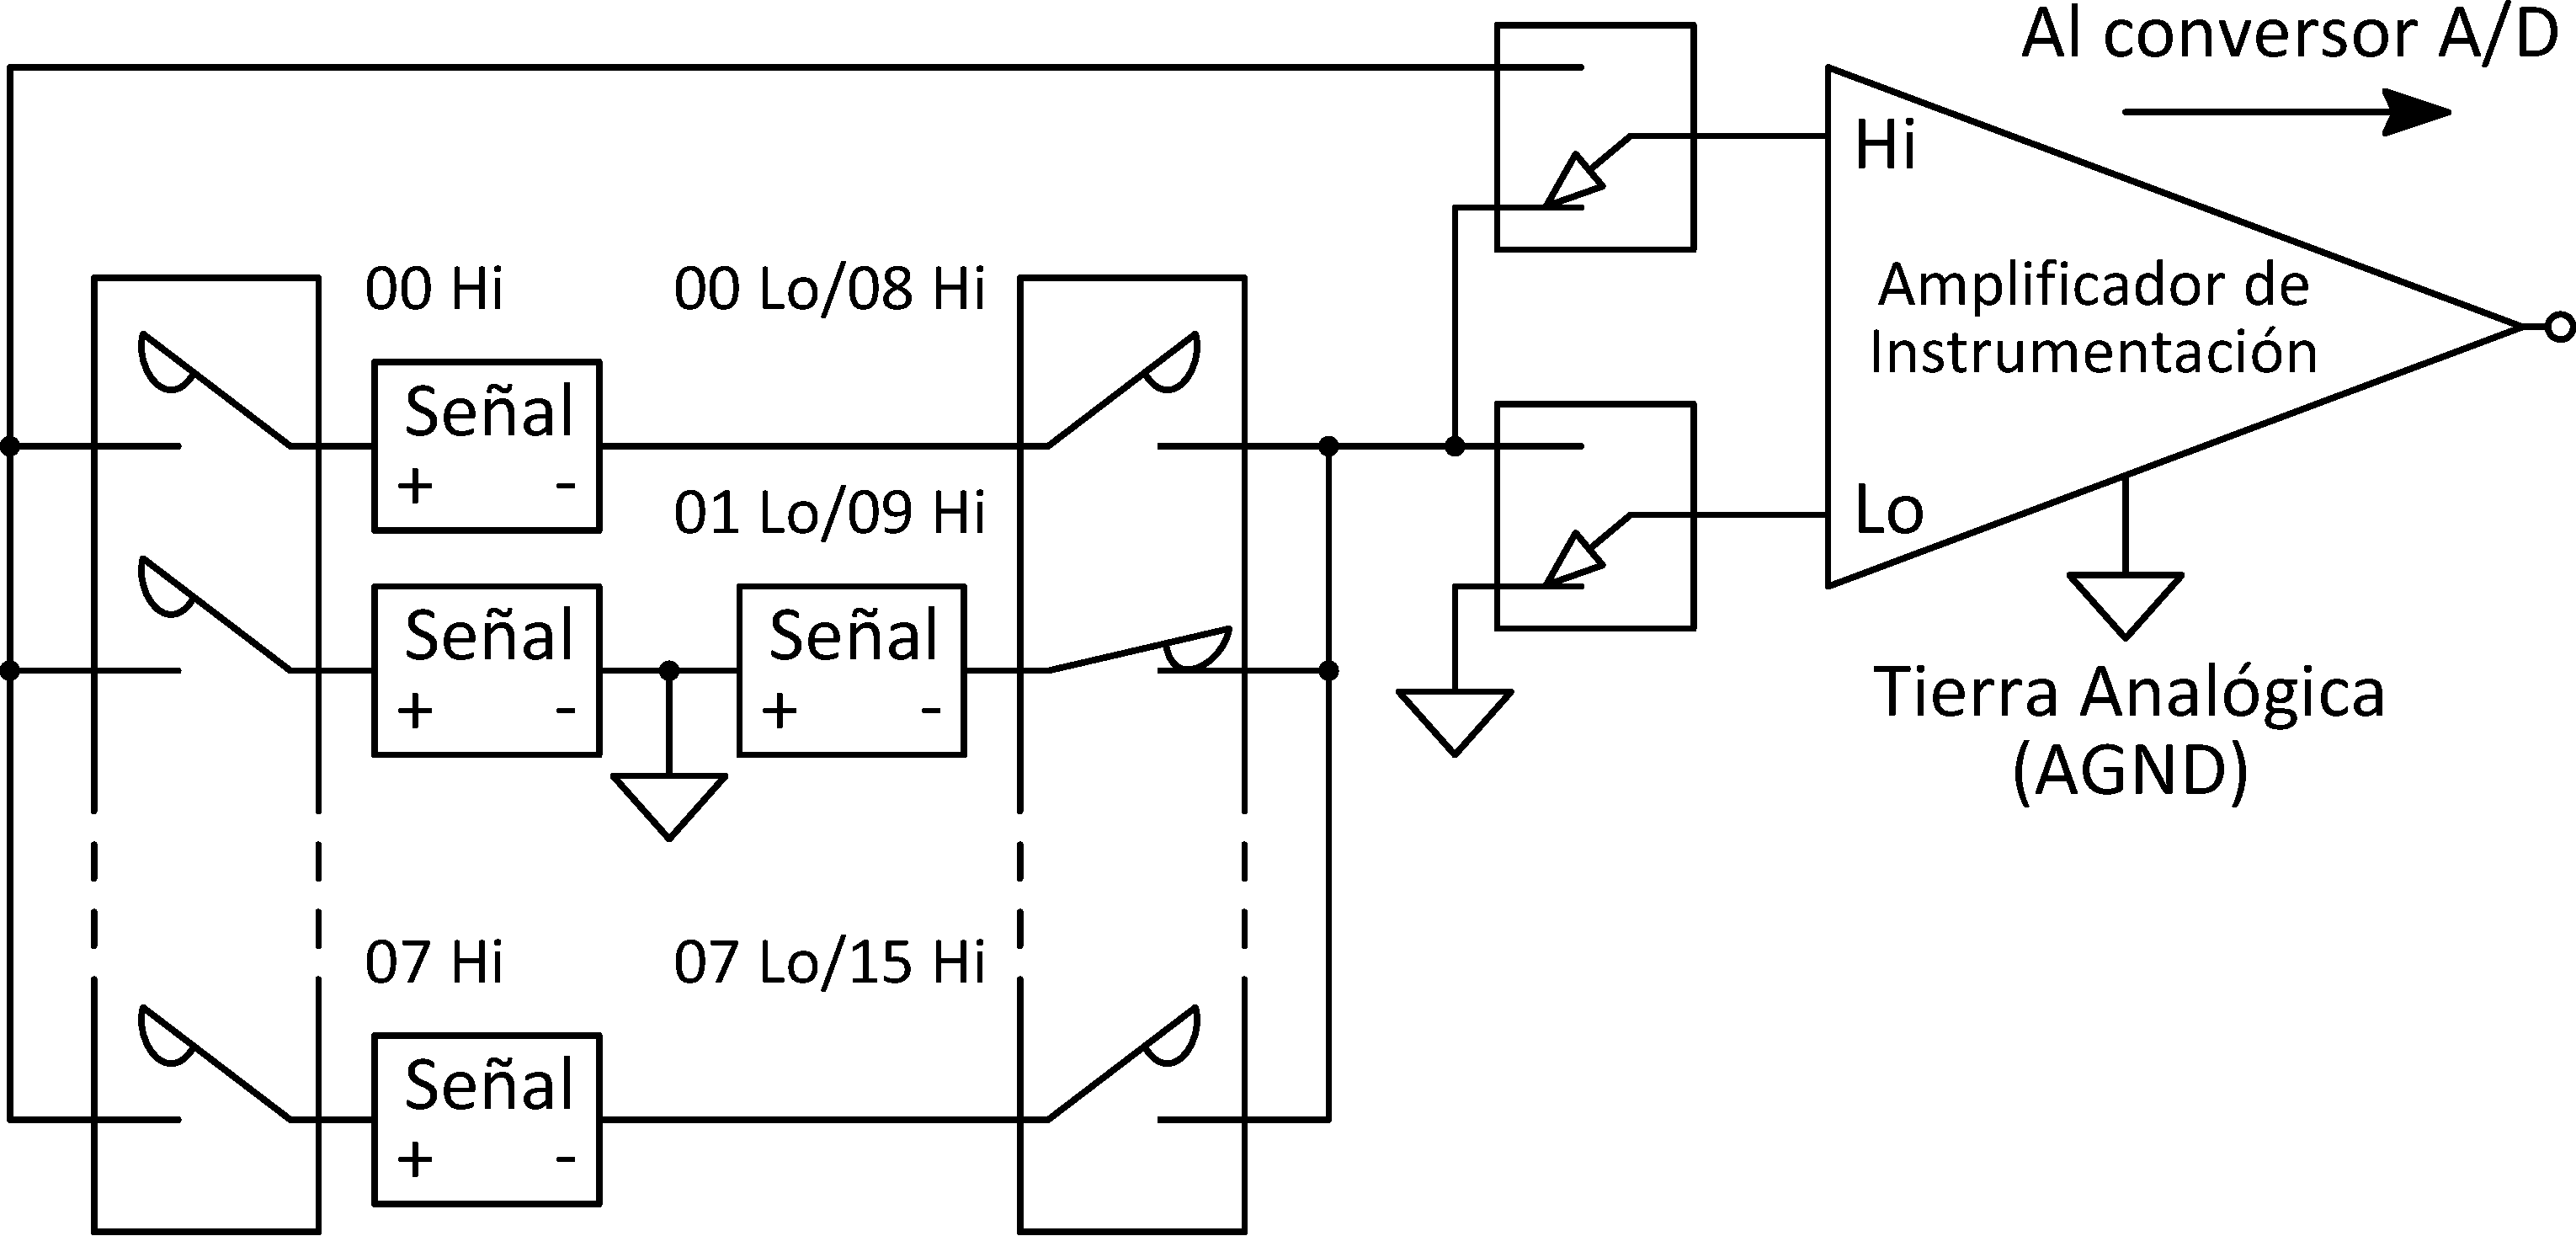
\includegraphics[height=.5\textheight, keepaspectratio=true]{chapter02-01.pdf}
	\end{center}
	\caption{Elementos que intervienen en el funcionamiento de la \datx{}}
	\label{fig:toolbox-components}
\end{figure}

\subsubsection{Objetos dispositivo}

Los objetos dispositivo permiten el acceso a subsistemas espec�ficos del hardware. Los objetos dispositivo soportados por la \datx{} son los objetos de entrada anal�gica o \emph{analog imput objects} (\textsc{ai}), los objetos de salida anal�gica o \emph{analog output objects} (\textsc{ao}) y los objetos de entrada/salida digital o \emph{digital \textsc{i/o} objects} (\textsc{dio}).

\begin{figure}[htbp]
	\begin{center}
		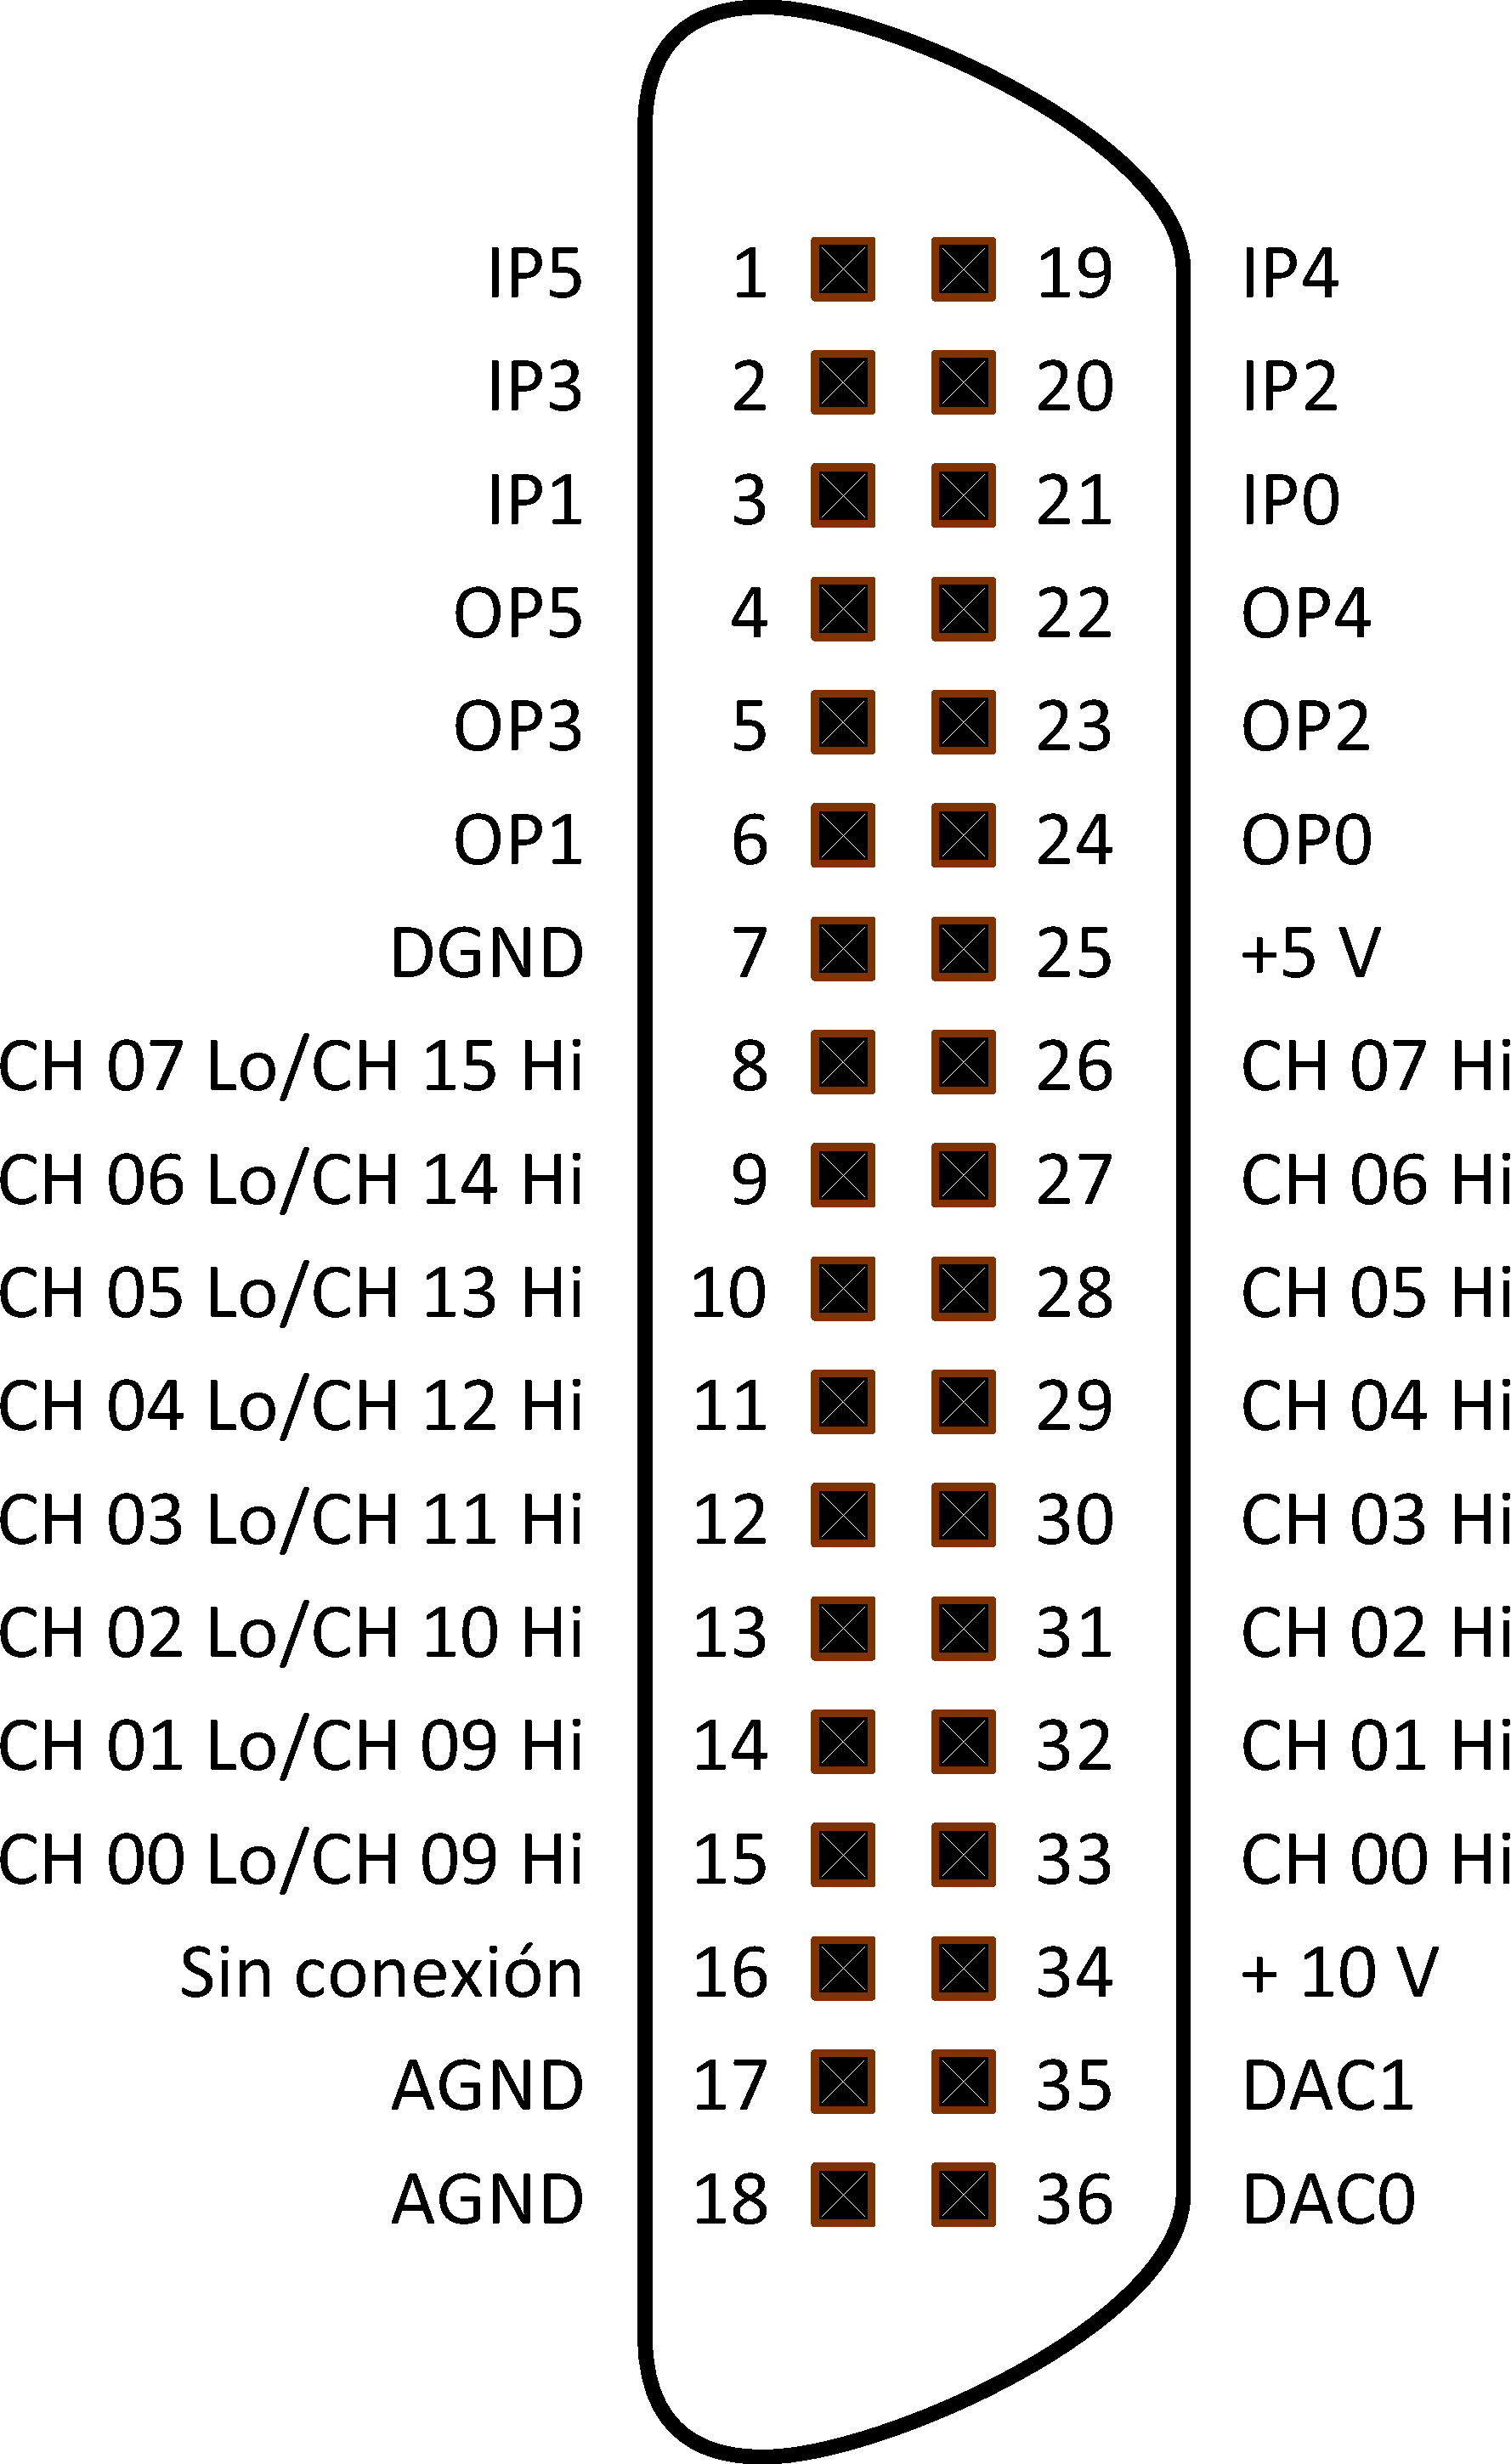
\includegraphics{chapter02-02.pdf}
	\end{center}
	\caption{Grafo que representa la comunicaci�n entre los subsistemas del hardware y los objetos dispositivo}
	\label{fig:subsystems-objects}
\end{figure}


\subsection{La sesi�n de adquisici�n de datos}

Una sesi�n completa de adquisici�n de datos consiste en cinco pasos:

\begin{enumerate}
	\item Crear el objeto dispositivo.
	\item A�adir canales al objeto dispositivo.
	\item Configurar las propiedades del objeto dispositivo y los canales a�adidos para controlar el comportamiento de la aplicaci�n de adquisici�n de datos.
	\item Adquirir los datos. % Iniciar la sesi�n de adquisici�n.
	\item Eliminar el objeto dispositivo. % Sesi�n de limpieza.
\end{enumerate}

Cada uno de los pasos se detalla en los puntos subsiguientes.


\subsubsection{Crear el objeto dispositivo}

% Utilizo la tabla para luego decir que como a mi me interesa la adquisici�n utilizare el comando analoginput nada m�s
Para crear un objeto dispositivo, se debe llamar a la funci�n de creaci�n apropiada o constructor. Como se muestra en el \vref{tab:constructors}, los constructores reciben un nombre particular en funci�n del tipo de objetos dispositivo que crean. Para iniciar una sesi�n de adquisici�n de datos anal�gicos es necesario un comando como el siguiente, \texttt{analoginput(`adaptador', ID)}.\par

\begin{lstlisting}[style=displayed, caption={[M�todo a seguir para crear un objeto dispositivo]M�todo que eval�a la existencia de un objeto dispositivo previo a la llamada de la aplicaci�n, en caso positivo lo hereda para su uso posterior, de lo contrario crea uno nuevo}, label={tab:constructor-example}]
	handles.ai = [];

	if ~isempty(daqfind)
		oldObj = daqfind;

		for i = 1:length(oldObj);
			auxStr = daqhwinfo(oldObj(i));
			auxNum = findstr(' ', auxStr.DeviceName) - 1;
			if strcmp('KPCI-3108', ...
				auxStr.DeviceName(1:auxNum)) && ...
				strcmpi('analoginput', auxStr.SubsystemType);
				handles.ai = oldObj(i);
				warning('El dispositivo est� en uso.');
				break
			end
		end

	end

	if isempty(handles.ai)
		try
			handles.ai = analoginput('keithley');
		catch
			errordlg('No pudo crearse el manejador de dispositivo.');
		end
	end
\end{lstlisting}

\begin{table}[htbp]
	\centering
	\begin{tabular}{l >{\tt}l}
		\toprule
		\multicolumn{1}{c}{Tipo de subsistema} & \multicolumn{1}{c}{\rm Constructor} \\
		\midrule
		Entrada anal�gica & analoginput(`adaptador', ID); \\
		\midrule
		Salida anal�gica & analogoutput(`adaptador', ID); \\
		\midrule
		Entrada / Salida digital & digitalio(`adaptador', ID); \\
		\bottomrule
	\end{tabular}
	\caption{Tipos de funci�n de creaci�n de acuerdo con el tipo subsistema al que se orienta el objeto dispositivo creado}
	\label{tab:constructors}
\end{table}

El argumento \texttt{id} es un indicador de dispositivo hardware. Se trata de un argumento opcional para tarjetas de sonido con \texttt{id} 0. El argumento \texttt{adaptador} requiere el nombre del adaptador de dispositivo hardware. A continuaci�n, en el \ref{tab:adaptors} se muestra una relaci�n con los adaptadores de dispositivo cuyo uso es m�s frecuente y el nombre de adaptador que debe introducirse como argumento de la llamada a \texttt{analoginput}. Por conveniencia se ha a�adido Keithley a esta lista.

\begin{table}[htbp]
	\centering
	\begin{tabular}{l >{\tt\qquad}l}
		\toprule
		\multicolumn{1}{c}{Fabricante de Hardware} & \multicolumn{1}{c}{\rm Nombre de adaptador} \\
		\midrule
		Advantech & advantech \\
		\midrule
		Measurement Computing & mcc \\
		\midrule
		National Instruments & nidaq \\
		\midrule
		Parallel port & parallel \\
		\midrule
		Microsoft Windows & winsound \\
		\midrule
		Keithley Instruments, Inc. & keithley \\
		\bottomrule
	\end{tabular}
	\caption{Argumento que debe emplearse en la llamada a \texttt{analoginput} en funci�n del fabricante}
	\label{tab:adaptors}
\end{table}


\subsubsection{A�adiendo canales}

Antes de poder utilizarse, deben a�adirse canales al objeto dispositivo. Para ello, debe emplearse la funci�n \texttt{addchannel}. Puede pensarse en un objeto dispositivo como un contenedor de grupos de canales y en los canales a�adidos a un objeto dispositivo como un grupo de canales. Si se desean a�adir dos canales al objeto dispositivo \texttt{objeto} puede utilizarse la siguiente llamada \texttt{cans = addchannel(objeto, 1:2);}.


\subsubsection{Configurando propiedades}

Puede controlarse el comportamiento de una sesi�n de adquisici�n de datos o de una aplicaci�n creada con tal prop�sito configurando las propiedades de los objetos dispositivo que intervienen en el proceso de adquisici�n y de los canales que dicho objeto contiene. Estas son las reglas principales en la configuraci�n de propiedades desde la \datx{}.

\begin{itemize}
	\item Los nombres de las propiedades pueden escribirse en may�sculas, min�sculas o combinaci�n de ambas.
	\item Los nombres de las propiedades pueden abreviarse como se mostrar� a continuaci�n. % Hay que confirmar que se explican las reglas de abreviatura
	\item La funci�n \texttt{set} aplicada a un objeto dispositivo ---\texttt{set(objeto)}--- devuelve todas las propiedades configurables de ese objeto. Si se llama a \texttt{set} utilizando como argumento un canal ---\texttt{set(objeto.Channel(�ndice)}---, la funci�n devolver� todas las propiedades configurables de dicho canal.
	\item La funci�n \texttt{get} devuelve todas las propiedades de un canal u objeto y el valor que toman en el momento en el que se llama a la funci�n si se emplea como �nico argumento dicho canal u objeto ---\texttt{get(objeto)}, \\ \texttt{get(objeto.Channel(�ndice)}---.
\end{itemize}

Se distinguen dos tipos de propiedades distintas asociadas a los canales contenidos en un objeto dispositivo.

\begin{itemize}
	\item \emph{Propiedades comunes} que se aplican a cada canal contenido en un objeto dispositivo.
	\item Y \emph{propiedades de canal} que pueden configurarse individualmente por canal.
\end{itemize}

Dentro de las propiedades comunes de los canales existen las \emph{propiedades b�sicas}, que se aplican a todos los subsistemas de un determinado tipo (\textsc{ai, ao, dio}); y \emph{propiedades espec�ficas de dispositivo} aplicables �nicamente al hardware espec�fico que se est� empleando.\par
Existen tres formas de configurar u obtener el valor de una propiedad: utilizando las funciones \texttt{set} y \texttt{get}; empleando la notaci�n de punto; o recurriendo a los nombres indexados.

\begin{itemize}
	\item La sintaxis de las funciones \texttt{get} y \texttt{set} es similar a la empleada en la herramienta de \matlab{} \emph{Handle Graphics}.
		\begin{lstlisting}[gobble=16]
			out = get(objeto, `SampleRate');
			set(objeto, `SampleRate', 11025)
		\end{lstlisting}
	\item La notaci�n de punto se emplea del siguiente modo:
		\begin{lstlisting}[gobble=16]
			out = objeto.SampleRate;
			objeto.SampleRate = 11025;
		\end{lstlisting}
	\item Por �ltimo, los nombres indexados permiten asociar un nombre descriptivo a cada canal. Por ejemplo para asociar el nombre \texttt{Can1} con el primer canal contenido en \texttt{objeto} debe procederse como se enuncia a continuaci�n.
		\begin{lstlisting}[gobble=16]
			set(objeto.Channel(1), `ChannelName', `Can1');
			out = objeto.Can1.UnitsRange;
			objeto.Can1.UnitsRange = [0, 10];
		\end{lstlisting}
\end{itemize}


\subsubsection{Adquisici�n de datos}

La adquisici�n de datos puede dividirse en tres tareas b�sicas: iniciar el objeto dispositivo; registrar datos y detener el objeto dispositivo.\par
La funci�n que se utiliza para iniciar un objeto dispositivo es la funci�n \texttt{start}, p.e. para iniciar el objeto dispositivo \texttt{objeto} habr�a que llamar a la funci�n de esta forma \texttt{start(objeto)}. Tras iniciar un objeto su propiedad \textsf{Running} pasa de manera autom�tica al valor \textsf{On}.\par
No obstante haber iniciado el dispositivo, este no empieza a registrar datos hasta que no ocurre un trigger o disparo. Hay diversos tipos de trigger, en el \vref{tab:triggers} se muestran aquellos soportados por todos los dispositivos. Tras un trigger el dispositivo hardware inicia la adquisici�n de datos y la propiedad \textsf{Logging} del objeto dispositivo asociado conmuta al estado \textsf{On}.

\begin{table}[htbp]
	\centering
	\begin{threeparttable}
	\begin{tabulary}{.9\linewidth}{>{\sf}c L}
		\toprule
		{\rm Tipo de disparo} & \multicolumn{1}{c}{Descripci�n} \\
		\midrule
		Inmediato & El disparo ocurre justo despu�s de la llamada a \texttt{start}. Este es el tipo de trigger predeterminado. \\
		\midrule
		Manual & El disparo ocurre despu�s de llamar manualmente a la funci�n \texttt{trigger}. \\
		\midrule
		Software & El disparo sucede cuando se detecta una se�al que satisface una determinada condici�n especificada de antemano. El objeto dispositivo debe disponer de m�s de un canal que har� las veces de la se�al de disparo. Debe especificarse, como es obvio, que canal act�a como fuente del disparo. \\
		\midrule
		Reloj interno\tnote{\rm a} & Por a�adidura, la \kpci{} cuenta con la posibilidad de recibir el disparo de la fuente de reloj interna. \\
		\bottomrule
	\end{tabulary}
	\begin{TableNotes}
		\tnotetext{a}{Se ha a�adido esta caracter�stica de la \kpci{} a la lista original.}
	\end{TableNotes}
	\end{threeparttable}
	\caption{Tipos de disparo soportados por el hardware compatible con \matlab{} y una breve descripci�n de los mismos}
	\label{tab:triggers}
\end{table}

Por �ltimo, existen tres causas por las que un objeto dispositivo puede detenerse: \matlab{} detiene un objeto dispositivo iniciado una vez obtenidos los datos precisados por el usuario; al ocurrir un error de tiempo de ejecuci�n en relaci�n con la actividad de un objeto dispositivo �ste es detenido tambi�n; y tan s�lo resta el m�todo manual, que consiste en llamar a la funci�n \texttt{stop}, por ejemplo \texttt{stop(objeto)}.\par
Como se ha mencionado la m�quina virtual de adquisici�n de datos registra y controla los datos que extrae de un objeto dispositivo. Un usuario puede acceder a esos datos de dos formas diferentes:

\begin{itemize}
	\item La primera de ellas se conoce como previsualizar los datos. Se emplea con ese prop�sito la funci�n \texttt{peekdata}. Si, por ejemplo, se quisiese previsualizar 1000 muestras obtenidas con el objeto dispositivo \texttt{objeto}, la llamada a \texttt{peekdata} ser�a la siguiente: \texttt{out = peekdata(objeto, 1000);}. La funci�n \texttt{peekdata} devuelve el control a \matlab{} de inmediato y no elimina los datos previsualizados de la m�quina virtual de adquisici�n.
	\item En cualquier momento tras adquirir datos mediante un objeto dispositivo estos pueden extraerse de la m�quina virtual de adquisici�n mediante la funci�n \texttt{getdata}. Partiendo del ejemplo anterior, si se desea extraer 1000 muestras procedentes del objeto dispositivo \texttt{objeto}, esta es la llamada adecuada \texttt{out = getdata(objeto, 1000);}. Al contrario que la funci�n \texttt{peekdata}, \texttt{getdata} no devuelve el control a \matlab{} hasta haber extra�do todas las muestras solicitadas. Es evidente que las muestras extra�das dejar�n de estar disponibles en la m�quina virtual de adquisici�n.
\end{itemize}

Es importante se�alar que en cualquiera de los procedimientos descritos intentar acceder a m�s datos de los obtenidos en un determinado momento causar� un error que detendr� el funcionamiento del objeto dispositivo.


\subsubsection{Eventos y Callbacks}

Puede decirse que un evento sucede en un determinado instante despu�s de que una cierta condici�n se cumple. A menos que ocurra un error, en todas las sesiones de adquisici�n de datos debe producirse un evento de inicio, uno de disparo y uno de parada. Puede accederse a la informaci�n que transporta un evento mediante la propiedad \textsf{EventLog}:

\begin{lstlisting}
	Events = ai.EventLog;
	EventTypes = {Events.Types}
	EventTypes =
		`Start'    `Trigger'	`Stop'
\end{lstlisting}

Cuando se produce un evento, puede ejecutarse una funci�n de \emph{callback}. Es posible seleccionar una funci�n para un callback especificando como valor de la propiedad asociada a dicho callback el nombre de la funci�n (si �sta se encuentra en el mismo fichero *.m que contiene el c�digo que ejecuta la aplicaci�n que realiza la adquisici�n de datos), o el nombre del fichero *.m con el c�digo de la funci�n. As� mismo, pueden pasarse argumentos de entrada a la funci�n de callback asign�ndolos a la mencionada propiedad.\par
Por ejemplo, los siguientes comandos configuran \texttt{objeto} de forma que la funci�n \texttt{datadqcallback} se ejecute desde el fichero cuyo nombre est� compuesto por una ra�z id�ntica al nombre de la funci�n y con extensi�n *.m, cuando se produzca un evento de trigger o de parada durante la actividad del objeto dispositivo. Adem�s se pasa como argumento de la funci�n el valor de la propiedad \textsf{Running} de \texttt{objeto} en el momento del callback.

\begin{lstlisting}
	set(objeto, `TriggerFcn', @datadqcallback, objeto.Running)
	set(objeto, `StopFcn', @datadqcallback, objeto.Running)
\end{lstlisting}

Un segundo ejemplo, este extra�do del c�digo fuente de la aplicaci�n de control muestra como pasar argumentos a la funci�n de callback y cu�l es la sintaxis de la definici�n de la misma.

\begin{lstlisting}[style=displayed, caption={Configuraci�n de \emph{callback} para responder a eventos en la sesi�n de muestreo, la funci�n de \emph{callback} recibe un argumento}]
	set(handles.ai, 'TriggerType', 'Immediate', 'TimerFcn', '', ...
		'SamplesAcquiredFcn', {@localDaqCallback, gcbo});

				[...]

	function localDaqCallback(obj, event, hObject)
		handles = guidata(hObject);
		EventType = event.Type;

		switch lower(EventType)
			case 'samplesacquired'

				[...]

			case 'timer'

				[...]

		end
\end{lstlisting}\vspace*{-20pt}

\subsubsection{Suprimiendo y borrando las trazas de los objetos dispositivo}

La funci�n \texttt{delete} elimina el objeto dispositivo especificado de la m�quina virtual de adquisici�n, pero no del espacio de trabajo de \matlab{}, ---\texttt{delete(objeto)}---. Tras una llamada semejante \texttt{objeto} sigue apareciendo en el espacio de trabajo de \matlab{}, pero se trata de un objeto inv�lido desde el momento en el que deja de encontrarse ligado al hardware. Deben suprimirse los objetos dispositivo faltos de validez con el comando \texttt{clear}, p.e., \texttt{clear objeto}.\par
Si se suprime un objeto dispositivo del espacio de trabajo de \matlab{} no deja de existir en la m�quina virtual. Para poder recuperar objetos borrados accidentalmente puede utilizarse la funci�n \texttt{daqfind}.

\begin{lstlisting}
	out = daqfind;
	ai = out(1);
\end{lstlisting}


\section{Prueba de funcionamiento}\label{sec:working-test}

En el apartado anterior se han dado las claves necesarias para desarrollar un software como el empleado en este proyecto, no obstante, en este documento no se contempla entrar con mayor detalle en el c�digo desarrollado m�s all� de lo que hasta ahora se ha hecho. Para obtener mayor informaci�n sobre las caracter�sticas y funcionalidades de la aplicaci�n desarrollada el lector puede remitirse al ap�ndice \vref{chap:apendixA}, en el cual se ha desarrollado lo que podr�a considerarse un manual de usuario para dicha aplicaci�n.\par
Para comprobar el buen funcionamiento del dispositivo de adquisici�n anal�gica y, en general, del sistema de representaci�n de se�ales, se ha dise�ado un experimento que pretende evaluar el comportamiento del conjunto por medio de la comparaci�n, utilizando como referencia un osciloscopio de laboratorio.\par
% El p�rrafo de abajo es complicado de leer y no da una idea clara de lo que quiero expresar. M�s o menos lo que hago es aprovechar el montaje que hago para la prueba y matar dos p�jaros de un tiro, certificar que el aparato funciona y dejar por escrito los pasos que deben seguirse al realizar cualquier experimento con el mismo. No creo que sea la mejor idea. Puedo utilizar alg�n art�culo de la web de Tom's Hardware como muestra de como tengo que exponer el experimento: una introducci�n en la que digo lo que estoy evaluando del aparato (si pueden manejarse de tanta frecuencia, que formas reconoce, como funciona el trigger en distintas situaciones de offset y desfase.. .); despu�s debo dar una tabla con la configuraci�n b�sica de los experimentos (tipos de se�ales empleadas, frecuencias, referencias a las fuentes, quiz� sondas.. .); caracter�sticas vistas en los experimentos del dispositivo y de la referencia; conclusiones que se extraen.
% Tom da tambi�n, entre la intro y la configuraci�n de la prueba, una breve descripci�n de las placas y una comparaci�n de las mismas (puertos disponibles de tal tipo, controladores de lo otro.. .) quiz� pueda hacer algo parecido, decir cuantas sondas pueden conectarse al osciloscopio, velocidades de muestreo, y ese tipo de cosas.
Para completar esta parte del documento se ha considerado conveniente la inclusi�n de �ste apartado cuyo objetivo es cubrir desde un punto de vista pr�ctico cual es el procedimiento a seguir durante una prueba que se realice mediante el sistema propuesto en este \textsc{pfc} y cuales son los resultados de dicha prueba en comparaci�n con los de un osciloscopio de laboratorio. La opci�n elegida para dar fin a tal prop�sito es la de documentar un ejercicio est�ndar a modo de ejemplo pr�ctico.\par


\subsection{Montaje del dispositivo de medida}

Puede completarse el montaje del sistema siguiendo un sencillo procedimiento que contempla una serie de pasos expuestos a continuaci�n.

\begin{enumerate}
	\item En primer lugar debe conectarse la interfaz ampliada desarrollada para el proyecto (v�ase la \vref{subsec:connection-box}) a los dos conectores mini-\textsc{d} provistos por la \kpci{}. Los dos conectores deben encontrarse en la parte posterior de la carcasa del ordenador al que se haya conectado la tarjeta. Los conectores hembra de la tarjeta y los conectores macho de los cables de la caja de conexiones est�n etiquetados con las palabras \emph{analog} y \emph{digital}, deben conectarse los cables de forma que las etiquetas en los conectores coincidan.
	\item Despu�s es necesario establecer conexiones entre las fuentes de las se�ales que se quiera intervengan en el proceso de adquisici�n anal�gica y la caja de conexiones. Para ello se recomienda emplear sondas terminadas por un lado en conector macho banana o coaxial y por otro en conector de tipo cocodrilo. La terminaci�n en conector de tipo banana o coaxial debe insertarse en uno de los conectores tipo hembra que la caja de conexiones dispone a tal efecto, por ejemplo, en el conector que comunica con el puerto anal�gico \textsc{ch00} de la tarjeta\footnote{Se recomienda en cualquier caso emplear los puertos anal�gicos \textsc{ch00} y \textsc{ch08} de la \kpci{} ya sea desde la interfaz banana o desde la interfaz coaxial.}. Y la terminaci�n en cocodrilo a la fuente de la se�al anal�gica de inter�s.
	\item Tras el paso anterior debe encenderse el ordenador y, una vez se ha accedido al sistema, lanzar \matlab{}.
	\item Por �ltimo, ya en la consola de \matlab{}, acceder al directorio en el que se encuentren los archivos \texttt{single-channel.m} y \texttt{single-channel.fig} y lanzar la aplicaci�n de control.
\end{enumerate}


\part{Ensayos no destructivos con ultrasonidos}

\chapter{Aplicaci�n para el control de la tarjeta}

\section{Introducci�n}

Desde los inicios de este proyecto lo que se ha pretendido es emplear un sistema de adquisici�n de se�ales como un osciloscopio digital. Para ello son necesarios la tarjeta de adquisici�n y un software que permita al usuario controlar el dispositivo desde una interfaz intuitiva y visualizar los resultados de forma sencilla.


\subsection{Funcionamiento de un osciloscopio}

Como se ha mencionado, el modelo de funcionamiento utilizado como referencia en el desarrollo de la aplicaci�n de control es el de un osciloscopio digital. Por ello, y en base a las conclusiones extra�das durante la realizaci�n de este proyecto, se ha cre�do conveniente explicar de forma breve como funcionan de manera habitual este tipo de osciloscopios.\par
Los osciloscopios anal�gicos emplean un tubo de rayos cat�dicos y un monitor de f�sforo para generar una imagen de la se�al. El cursor que el tubo dibuja en el monitor lo va barriendo de izquierda a derecha con periodicidad, y su posici�n vertical refleja en cada momento el valor de tensi�n de la se�al el�ctrica que entra al osciloscopio. El monitor preserva durante breves instantes una traza del cursor y as� se forma la imagen que representa a la se�al.\par
En la actualidad suelen emplearse osciloscopios digitales. El procedimiento que sigue un osciloscopio digital para representar se�ales es completamente diferente al que siguen los osciloscopios anal�gicos. No existe ning�n cursor, se generan fotogramas de la se�al\footnote{En realidad, los osciloscopios digitales modernos pueden representar por pantalla varias se�ales simult�neamente.} en seguimiento, im�genes completas que cubren la pantalla entera con un fragmento de se�al. Una vez aparece una imagen por pantalla permanece est�tica hasta que una nueva imagen la sustituye. La dimensi�n temporal de la representaci�n determina en teor�a cuanto debe esperar el osciloscopio desde que se muestra por pantalla una imagen hasta que se puede generar la siguiente. La espera resulta evidente puesto que la se�al no se conoce de antemano. Al contrario que ocurre con los osciloscopios anal�gicos que representan la se�al en tiempo real, si se desea representar por pantalla un fragmento de la se�al de una determinada duraci�n el osciloscopio debe esperar hasta que transcurra dicho periodo de tiempo. En otras palabras, aparece un retardo que depende exclusivamente de la duraci�n del fragmento de se�al necesario para cubrir la ventana del osciloscopio, o lo que es lo mismo, el retardo es independiente de otros par�metros como son la velocidad de muestreo o la potencia de procesado del osciloscopio.\par
Este modo de proceder tiene un inconveniente. El objetivo de un osciloscopio es mostrar en cada momento como es la forma de la se�al, si el retardo introducido es demasiado alto el osciloscopio deja de ser eficaz pues la informaci�n que proporciona cada imagen es obsoleta. Problema que se ve agravado por la posibilidad de configurar el eje de tiempos. As� es, tanto los osciloscopios anal�gicos (variando la frecuencia de barrido del cursor) como los osciloscopios digitales, permiten que el usuario modifique la cantidad de tiempo que refleja el eje horizontal de la representaci�n, pudiendo ser �sta mayor o menor. A efectos pr�cticos, en los osciloscopios digitales el tiempo abarcado por el eje temporal act�a como el inverso de la frecuencia de refresco del monitor, por tanto, cuanto mayor sea ese tiempo con mayor lentitud se suceder�n las im�genes y habr� un mayor desfase entre la se�al y la representaci�n de �sta.


\subsection{Modos de representaci�n en los osciloscopios digitales}

Para evitar que en determinadas configuraciones del eje temporal del osciloscopio el retardo sea excesivo, la mayor�a de estos dispositivos implementan dos modos de funcionamiento: el modo convencional que se aplica en situaciones en las que el retardo no se considera importante; y una especie de modo continuo. Existen dos criterios que se siguen de manera habitual para diferenciar en que momento es m�s apropiado el uso de uno u otro modo: % En cierto modo esa es una forma de configurar el retardo o el volumen de im�genes mostradas por segundo en un osciloscopio digital. M�s tiempo transcurrir� entre una imagen y la siguiente. M�s anticuada ser� la informaci�n mostrada por pantalla. En el cual la forma de representar se asemeja a la que se da en osciloscopios anal�gicos.

\begin{itemize}
	\item El primer criterio eval�a el correcto funcionamiento del modo convencional. Como se ver� m�s adelante, el modo convencional de representaci�n en un osciloscopio requiere que la cantidad de im�genes que salen por pantalla cada segundo sea lo suficiente grande como para que se simule el movimiento. Por tanto para satisfacer el primer criterio, la tasa de refresco del monitor del osciloscopio debe superar las veintis�is im�genes por segundo o encontrarse alrededor de esta cifra.
	\item El segundo criterio est� relacionado con la funci�n de disparo que se da en el modo convencional de representaci�n. Para poder efectuar correctamente el disparo sobre se�ales de baja frecuencia, al generar cada imagen el osciloscopio debe haber registrado al menos un ciclo de la se�al pertinente\footnote{En la pr�ctica se necesita algo m�s de un ciclo de una se�al para poder garantizar el correcto disparo de �sta. Sin embargo, es com�n conseguir disparar una se�al aunque la configuraci�n del eje de tiempos del osciloscopio permita s�lo obtener una fracci�n del ciclo completo de esa se�al durante la realizaci�n de cada fotograma.}. Lo cual reduce la tasa m�nima de refresco a la frecuencia de la se�al m�s lenta que se desee representar de forma correcta en el modo convencional de representaci�n del osciloscopio.
\end{itemize}

Como puede verse el segundo criterio es m�s restrictivo pues depende de la frecuencia de la se�al y �sta puede ser en efecto inferior a un hercio, es por ello que se emplea habitualmente. Siendo as�, la tasa de refresco m�nima que se permite en el modo convencional en la gran mayor�a de dispositivos y que se ha adoptado para el software de control, es de cinco im�genes por segundo (5 Hz). Cuando se configura un osciloscopio en el modo convencional para que trabaje a esta tasa de refresco es habitual poder visualizar se�ales de frecuencia cercana a 1 Hz, sin embargo la representaci�n se optimiza para configuraciones en las que el osciloscopio muestra, al menos, veinticinco im�genes por segundo, lo cual es apropiado para se�ales con una frecuencia m�nima de 50 Hz. Si la configuraci�n del eje de tiempos del osciloscopio obligara al dispositivo a trabajar con una frecuencia de refresco inferior a la especificada, autom�ticamente conmuta para funcionar en el modo continuo.


\subsubsection{Representaci�n en modo continuo}

Una vez visto cual es la frecuencia umbral a la que el dispositivo conmuta entre los dos modos, debe explicarse que diferencia un modo de funcionamiento de otro. Para ello se expone a continuaci�n cuales son los fundamentos de uno y otro modo. La representaci�n en \emph{modo continuo} es, por decirlo as�, ininterrumpida. La imagen de la se�al de inter�s se desplaza de derecha izquierda a medida que transcurre el tiempo. Para lograr este efecto se aumenta la frecuencia de refresco a expensas de que, como es sabido, el fragmento de se�al obtenido para cada imagen no cubrir� la pantalla al completo. Ocurre as� por que la frecuencia de refresco es muy alta para el eje temporal que representa una gran cantidad de tiempo, por tanto, entre dos im�genes no transcurre el tiempo abarcado por la dimensi�n horizontal de la representaci�n. La primera imagen sit�a el fragmento de se�al que se ha digitalizado en el extremo derecho de la representaci�n, el resto se deja en blanco. Con cada nueva imagen se desplaza el fragmento de se�al representado hasta el momento el suficiente espacio hacia la izquierda como para incorporar un nuevo fragmento de se�al. As� la porci�n de se�al representada aumenta cada vez m�s hasta que el extremo izquierdo de la figura alcanza el margen izquierdo de la ventana del osciloscopio. Cuando esto ocurre, empieza un desplazamiento c�clico, al incorporar un nuevo fragmento de se�al a la derecha se retira un fragmento de la misma proporci�n temporal al otro extremo. La alta tasa con la que aparecen las im�genes por pantalla garantizan que la representaci�n siga casi en tiempo real ---por lo menos as� lo percibe el ojo humano--- a la se�al verdadera. Debe notarse, no obstante, que este m�todo de representaci�n no es adecuado para se�ales de alta frecuencia pues aunque el eje temporal abarque un tiempo mayor, la dimensi�n del monitor obviamente no var�a y las se�ales de alta frecuencia aparecer�n en exceso comprimidas.\par


\subsubsection{Representaci�n en modo convencional}

El \emph{modo convencional} de representaci�n es algo m�s complicado. Como se ha declarado con anterioridad en este mismo apartado, la representaci�n convencional basa su funcionamiento en im�genes que muestran fragmentos de se�al que cubren la dimensi�n temporal de la ventana del osciloscopio y que se suceden unas a otras con presteza. La idea que persigue este m�todo es la de conseguir algo semejante a una pel�cula de la se�al. Para ello, no es s�lo suficiente con que aparezcan muchas im�genes por segundo en el monitor del osciloscopio, esas im�genes deben estar de alg�n modo relacionadas entre s�. Si las im�genes que aparecen en el monitor son de forma consecutiva muy diferentes es probable que no pueda discernirse nada claro, y de nada valdr� la representaci�n.\par
	Ah� es donde entra en juego el procesado y la funci�n de disparo de un osciloscopio digital. Cuando un fragmento suficientemente largo como para cubrir la ventana de representaci�n se digitaliza y se almacena en memoria, empieza el procesado digital del mismo. El prop�sito del procesado es, ente otras cosas, eliminar las posible componente en continua, averiguar informaci�n adicional de la se�al en la medida de lo posible, como p.e. su valor de pico a pico, o implementar una funci�n de disparo. La funci�n de disparo del osciloscopio persigue alinear los ejes verticales de la ventana donde se representa con los cruces de la se�al con respecto a un determinado valor de umbral que puede ser configurado por el usuario. La idea es alinear al menos el cruce m�s centrado de cada fragmento de se�al con el eje de abscisas que corta en dos mitades la ventana. Para conseguirlo, durante el procesado se detectan todos los cortes de la se�al con el umbral y despu�s se desplaza el fragmento de se�al para que el corte m�s centrado case con el eje de abscisas. Si la se�al es peri�dica las variaciones entre un fotograma y el siguiente ser�n m�nimas, puesto que ambos estar�n alineados, y se simular� con �xito el movimiento.\par
	No obstante, la necesidad de desplazar el fragmento de se�al que va a representarse presenta un inconveniente importante. Para poder desplazar el fragmento de se�al y que se cubra completamente la ventana del osciloscopio su duraci�n, la del fragmento de se�al digitalizado, debe ser superior al tiempo reflejado en el eje de tiempos de la ventana. De lo contrario la se�al aparecer� truncada, se mostrar� un espacio en blanco y, con una tasa de refresco alta, la visualizaci�n ser� confusa. Desplazar fragmentos de se�al implica dos cosas: por un lado el osciloscopio debe esperar m�s tiempo para refrescar la pantalla, es decir, se reduce la tasa de refresco para una misma configuraci�n del eje de tiempos; y por otro, al tener para representar un fragmento de se�al de mayor duraci�n que la reflejada por el eje temporal de la ventana parte del fragmento queda ahora fuera de la representaci�n.\par
	Este inconveniente se ve paliado por el hecho de que el modo convencional contempla en principio trabajar con se�ales de alta frecuencia. Estas se�ales cambian de forma tan r�pida que de no ser por el disparo ser�a imposible observar los cambios. Por otro lado puede seleccionarse que informaci�n que se muestra por pantalla accionando un control de offset temporal o modificando el valor de umbral de disparo y, generalmente, la p�rdida de informaci�n a causa del disparo no es significativa.


\section{Elaboraci�n del software de control}


\subsection{Elecci�n del entorno de desarrollo}

El lenguaje o, mejor dicho, plataforma que se ha empleado para el desarrollo del software de control es \matlab{}, la raz�n, su inmejorable compatibilidad con el hardware disponible. A partir de ah�, los componentes de \matlab{} que se han empleado para conseguir que el software de control gozase de las caracter�sticas previstas por los objetivos del proyecto son dos: el entorno de desarrollo de interfaces gr�ficas de usuario (\textsc{gui}) de \matlab{}, m�s conocido como \textsc{guide} (\emph{graphical user interface development environment}); y el \emph{Data Acquisition Toolbox} de \matlab{}. El primero de ellos se ha empleado para, como su nombre indica, crear la interfaz que comunica el dispositivo con el usuario. Esta comunicaci�n se hace a trav�s del segundo de los componentes mencionados, �ste permite, mediante comandos de \matlab{} que pueden incluirse en rutinas o llamarse por separado, manejar el dispositivo ---convocarlo a muestrear, configurar sus propiedades--- y administra autom�ticamente los resultados almacen�ndolos en b�ffers situados en la memoria vol�til del ordenador, haci�ndolos de este modo accesibles al administrador de la tarjeta.\par




\end{document}
